\section{各要素での具体的な行列について}
\numberwithin{equation}{subsection}
\subsection{基底関数について}
まずは基底関数$\psi$について基本ルールについておさらいしておこう.ここでは,2次元での基底関数について考えるが,1次元や3次元についても引数の変更によって同様の議論ができる.
\begin{NoteBox}{基底関数の基本ルール}{Rule_of_basis_function}
  \begin{equation}
    \label{Eq:shape-func-rule-1}
    \psi_i\pab{x_j, y_j} = \delta_{ij}
  \end{equation}
  \begin{equation}
    \label{Eq:shape-func-rule-2}
    \sum_{i=1}^{N_\mathrm{basis}}\psi_i\pab{x, t} = 1
  \end{equation}
  \small
  $\psi$:基底関数,$N_\mathrm{basis}$:基底関数の数,$\delta_{ij}$:クロネッカーのデルタ
\end{NoteBox}

\subsection{熱伝導マトリックスについて}
$\mat{R}$マトリックスについて考える.$\mat{R}$マトリックスは熱伝導率マトリックスであり,等方性の有無によって次のようになる.
\begin{equation}
  \mat{R} =
  \begin{cases}
    \begin{bmatrix}
      \lambda_{xx} & \lambda_{xy}\\
      \lambda_{yx} & \lambda_{yy}
    \end{bmatrix}\qquad\quad &\text{(Anisotropic material)}\\[10mm]
    \begin{bmatrix}
      \lambda & 0\\
      0       & \lambda
    \end{bmatrix}\qquad\quad &\text{(Isotropic material)}
  \end{cases}
\end{equation}
また土壌の場合$\lambda_{xy}=\lambda_{yx}$なのでAnisotropicな$\mat{R}$マトリックスは次のように書き換えられる.
\begin{equation}
  \mat{R} =
  \begin{bmatrix}
    \lambda_{xx} & \lambda_{xy}\\
    \lambda_{xy} & \lambda_{yy}
  \end{bmatrix}
\end{equation}
\subsection{三角形一次要素}
基底関数の存在を認めれば,三角形要素内の温度分布は次のようになる.
\begin{equation}
  T\pab{x,y}=\psi_1\pab{x,y}T_1+\psi_2\pab{x,y}T_2+\psi_3\pab{x,y}T_3
\end{equation}
温度の代わりに座標を代入すると,
\begin{subequations}
  \label{Eq:tri-basis}
  \begin{align}
    x &= \psi_1 x_1 + \psi_2 x_2 + \psi_3 x_3\\
    y &= \psi_1 y_1 + \psi_2 y_2 + \psi_3 y_3
  \end{align}
  さらに基底関数の基本ルールより,基底関数の和は常に1であるので,
  \begin{equation}
    \psi_1 + \psi_2 + \psi_3 = 1
  \end{equation}
\end{subequations}
\eqref{Eq:tri-basis}式の関係を用いれば次の連立方程式を得る.
\begin{equation}
  \begin{bmatrix}
    1 & 1 & 1\\
    x_1 & x_2 & x_3\\
    y_1 & y_2 & y_3
  \end{bmatrix}
  \begin{bmatrix}
    \psi_1\pab{x,y}\\ \psi_2\pab{x,y}\\ \psi_3\pab{x,y}
  \end{bmatrix}
  =
  \begin{bmatrix}
    1\\ x\\ y
  \end{bmatrix}
\end{equation}
よって,各要素の面積を$A_m$とすれば,
\begin{align}
  \psi\pab{x,y}=\dfrac{1}{2A_m}\pab{a_{m}+b_{m}x+c_{m}y}
\end{align}
となり,基底関数の各係数はTable~\ref{tab:tri-basis-coef}のようになる.
\begin{table}[]
  \centering
  \caption{基底関数の係数}
  \label{tab:tri-basis-coef}
  \begin{tabular}{@{}cccc@{}}
  \toprule
           & $a$             & $b$       & $c$       \\ \midrule
  $\psi_1$ & $x_2y_3-x_3y_2$ & $y_2-y_3$ & $x_3-x_2$ \\
  $\psi_2$ & $x_3y_1-x_1y_3$ & $y_3-y_1$ & $x_1-x_3$ \\
  $\psi_3$ & $x_1y_2-x_2y_1$ & $y_1-y_2$ & $x_2-x_1$ \\ \bottomrule
  \end{tabular}
\end{table}\\
ここで,$\mat{B}$マトリックスについて考える.$\mat{B}$マトリックスは基底関数の導関数を並べた行列である.
\begin{equation}
  \mat{B}=
  \begin{bmatrix}
    \displaystyle\pdv{\psi_1}{x} & \displaystyle\pdv{\psi_2}{x} & \displaystyle\pdv{\psi_3}{x}\\
    \displaystyle\pdv{\psi_1}{y} & \displaystyle\pdv{\psi_2}{y} & \displaystyle\pdv{\psi_3}{y}
  \end{bmatrix}
  = \dfrac{1}{2A_m}
  \begin{bmatrix}
    b_1 & b_2 & b_3\\
    c_1 & c_2 & c_3
  \end{bmatrix}
\end{equation}
$\mat{R}$マトリックスがIsotropicであれば,要素中の熱伝導率の平均$\bar{\lambda}$を用いると
\begin{equation}
  \iint_{\Omega^e}\mat{B}^\top\mat{R}\mat{B}\odif{\Omega^e}=\dfrac{\bar{\lambda}}{4A_m}
  \begin{bmatrix}
    b_1 b_1 + c_1 c_1 & b_1 b_2 + c_1 c_2 & b_1 b_3 + c_1 c_3\\
    b_2 b_1 + c_2 c_1 & b_2 b_2 + c_2 c_2 & b_2 b_3 + c_2 c_3\\
    b_3 b_1 + c_3 c_1 & b_3 b_2 + c_3 c_2 & b_3 b_3 + c_3 c_3
  \end{bmatrix}
\end{equation}
一方,$\mat{R}$マトリックスがAnisotropicであれば,
\begin{equation}
  \iint_{\Omega^e}\mat{B}^\top\mat{R}\mat{B}\odif{\Omega^e}=\dfrac{1}{4A_m}
  \begin{cases}
    \lambda_{xx}b_1b_1 + \lambda_{xy}(b_1c_1 + c_1b_1) + \lambda_{yy}c_1c_1 \qquad \text{Matrix}(1,1) \\
    \lambda_{xx}b_1b_2 + \lambda_{xy}(b_1c_2 + c_1b_2) + \lambda_{yy}c_1c_2 \qquad \text{Matrix}(1,2) \\
    \lambda_{xx}b_1b_3 + \lambda_{xy}(b_1c_3 + c_1b_3) + \lambda_{yy}c_1c_3 \qquad \text{Matrix}(1,3) \\
    \lambda_{xx}b_2b_1 + \lambda_{xy}(b_2c_1 + c_2b_1) + \lambda_{yy}c_2c_1 \qquad \text{Matrix}(2,1) \\
    \lambda_{xx}b_2b_2 + \lambda_{xy}(b_2c_2 + c_2b_2) + \lambda_{yy}c_2c_2 \qquad \text{Matrix}(2,2) \\
    \lambda_{xx}b_2b_3 + \lambda_{xy}(b_2c_3 + c_2b_3) + \lambda_{yy}c_2c_3 \qquad \text{Matrix}(2,3) \\
    \lambda_{xx}b_3b_1 + \lambda_{xy}(b_3c_1 + c_3b_1) + \lambda_{yy}c_3c_1 \qquad \text{Matrix}(3,1) \\
    \lambda_{xx}b_3b_2 + \lambda_{xy}(b_3c_2 + c_3b_2) + \lambda_{yy}c_3c_2 \qquad \text{Matrix}(3,2) \\
    \lambda_{xx}b_3b_3 + \lambda_{xy}(b_3c_3 + c_3b_3) + \lambda_{yy}c_3c_3 \qquad \text{Matrix}(3,3)
  \end{cases}
\end{equation}
ここで領域$\Omega^e$での基底関数の面積分を考えるためFig.~\ref{Fig:AreaCood}に示す面積座標を導入する.
\begin{figure}[H]
  \centering
  \begin{tikzpicture}[scale=1.5]
    \coordinate[label=below left:$O$](O)at(0,0);
    \coordinate(XS)at(-0.5,0);
    \coordinate(XL)at(8,0);
    \coordinate(YS)at(0,-0.5);
    \coordinate(YL)at(0,5);
    \draw[semithick,-{Latex}](XS)--(XL)node[below]{$x$};
    \draw[semithick,-{Latex}](YS)--(YL)node[left]{$y$};
    \coordinate[label=below:$P_1\pab{x_1,y_1}$](P1)at(0.85,0.75);
    \coordinate[label=right:$P_2\pab{x_2,y_2}$](P2)at(6,1.5);
    \coordinate[label=above:$P_3\pab{x_3,y_3}$](P3)at(3,4);
    \coordinate(P231)at(4,3.166666);
    \coordinate(P232)at(4.8,2.5);
    \coordinate(P)at(3.5,2.5);

    \draw(P1)--(P2)--(P3)--cycle;
    \draw(P)--(P1);
    \draw(P)--(P2);
    \draw(P)--(P3);

    \coordinate[label=below:$A_{12}^e$](G1)at($(P)!1/3!(P1)!1/3!(P2)$);
    \coordinate[label=above:$A_{23}^e$](G2)at($(P)!1/3!(P2)!1/3!(P3)$);
    \coordinate[label=above:$A_{31}^e$](G3)at($(P)!1/3!(P3)!1/3!(P1)$);

    \node[right, fill=white, inner sep=2pt, xshift=6pt, yshift=0pt] at (P) {$P{(\xi_1,\xi_2,\xi_3)}$};
    \draw (P1) node[circle, inner sep=2pt, fill=black]{};
    \draw (P2) node[circle, inner sep=2pt, fill=black]{};
    \draw (P3) node[circle, inner sep=2pt, fill=black]{};
    \draw (P) node[circle, inner sep=2pt, fill=black]{};
  \end{tikzpicture}
  \caption{面積座標の概念図}
  \label{Fig:AreaCood}
\end{figure}
$\triangle P_1 P_2 P_3 $は3つの三角形$\triangle P P_1 P_2 $,$\triangle P P_2 P_3 $,$\triangle P P_3 P_1 $に分割できる.これらを全体の三角形の面積$A^e$で割ったものを順に面積座標$\xi_1$,$\xi_2$,$\xi_3$と定義する.ただしそれぞれの三角形の面積は$A_{12}^{e}$,$A_{23}^{e}$,$A_{31}^{e}$とする.
\begin{subequations}
  \label{Eq:DefACoord}
  \begin{align}
    \xi_1 &= \frac{A_{12}^{e}}{A^e}\\
    \xi_2 &= \frac{A_{23}^{e}}{A^e}\\
    \xi_3 &= \frac{A_{31}^{e}}{A^e}
  \end{align}
\end{subequations}
また,$\xi$は次の関係があるのは自明である.
\begin{equation}
  \label{Eq:Relxi}
  \xi_1+\xi_2+\xi_3=1
\end{equation}
つまり,$\xi_1$と$\xi_2$が決定すると\eqref{Eq:Relxi}式より,自動的に$\xi_3=1-\xi_1-\xi_2$と決定でき$\xi_1$と$\xi_2$のみが独立変数となる.よって$0\leq\xi_2\leq 1-\xi_1$の条件下の領域$\Omega^e$内では$\forall P(x,y)\rightarrow P(\xi_1,\xi_2,1-\xi_1-\xi_2)$と表せる.ここで分割されたそれぞれの三角形の面積について考えることで,面積座標について考える.
\begin{subequations}
  \label{Eq:AreaSp}
  \begin{align}
    \xi_1 &= \frac{A_{12}^{e}}{A^e}\notag\\
    &=\frac{1}{2A^e}\bab{x\pab{y_2-y_3}+x_2\pab{y_3-y}+x_3\pab{y-y_2}}\notag\\
    &=\frac{1}{2A^e}\bab{\pab{x_2 y_3-x_3 y_2}+\pab{y_2-y_3}x+\pab{x_3-x_2}y}\notag\\
    &=\frac{1}{2A^e}\pab{a_1+b_1 x+c_1 y}\notag\\
    \label{Eq:AreaSp1j}
    &=\psi_1
  \end{align}
  同様に
  \begin{align}
    \xi_2 &= \frac{A_{23}^{e}}{A^e}\notag\\
    &=\frac{1}{2A^e}\bab{x\pab{y_3-y_1}+x_3\pab{y_1-y}+x_1\pab{y-y_3}}\notag\\
    &=\frac{1}{2A^e}\bab{\pab{x_3 y_1-x_1 y_3}+\pab{y_3-y_1}x+\pab{x_1-x_3}y}\notag\\
    &=\frac{1}{2A^e}\pab{a_2+b_2 x+c_2 y}\notag\\
    \label{Eq:AreaSp2j}
    &=\psi_2
  \end{align}
  \begin{align}
    \xi_3 &= \frac{A_{31}^{e}}{A^e}\notag\\
    &=\frac{1}{2A^e}\bab{x\pab{y_1-y_2}+x_1\pab{y_2-y}+x_2\pab{y-y_1}}\notag\\
    &=\frac{1}{2A^e}\bab{\pab{x_1 y_2-x_2 y_1}+\pab{y_1-y_2}x+\pab{x_2-x_1}y}\notag\\
    &=\frac{1}{2A^e}\pab{a_3+b_3 x+c_3 y}\notag\\
    \label{Eq:AreaSp3j}
    &=\psi_3
  \end{align}
\end{subequations}
よって三角形一次要素の基底関数は面積座標と一致する.そのため,面積座標上での面積分をすることによって,基底関数の積分を求めることができる.ここで\eqref{Eq:tri-basis-integral}式で示すように階乗を用いることで,面積座標での積分を解析的に求めることができる.
\begin{equation}
  \label{Eq:tri-basis-integral}
  \iint_{\Omega^e}\xi_1^p~\xi_2^q~\xi_3^r\odif{\Omega^e}=\dfrac{p!q!r!}{\pab{p+q+r+2}!}2A_m
\end{equation}
よって,\eqref{Eq:tri-basis-integral}式を用いれば,基底関数の積の積分は次のようになる.
\begin{equation}
  \iint_{\Omega^e}\vect{\psi}^\top\vect{\psi}\odif{\Omega^e}=\iint_{\Omega^e}
  \begin{bmatrix}
    \psi_1^2 & \psi_1\psi_2 & \psi_1\psi_3\\
    \psi_2\psi_1 & \psi_2^2 & \psi_2\psi_3\\
    \psi_3\psi_1 & \psi_3\psi_2 & \psi_3^2
  \end{bmatrix}\odif{\Omega^e}
  =\dfrac{A_m}{12}
  \begin{bmatrix}
    2 & 1 & 1\\
    1 & 2 & 1\\
    1 & 1 & 2
  \end{bmatrix}
\end{equation}
したがって,
\begin{equation}
  \iint_{\Omega^e}C_\mathrm{w}\vect{Q}_\mathrm{w}\vect{\psi}^\top\vect{\psi}\odif{\Omega^e}=C_\mathrm{w}\vect{Q}_\mathrm{w}\dfrac{A_m}{12}
  \begin{bmatrix}
    2 & 1 & 1\\
    1 & 2 & 1\\
    1 & 1 & 2
  \end{bmatrix}
\end{equation}
また,
\begin{align}
  &\iint_{\Omega^e} C_\mathrm{w} \vect{\psi}^\top \vect{q}^\top \mat{B} \odif{\Omega^e}\notag
  \\&=\dfrac{C_\mathrm{w}}{6}
  \begin{bmatrix}
    b_1q_x + c_1q_y & b_2q_x + c_2q_y & b_3q_x + c_3q_y\\
    b_1q_x + c_1q_y & b_2q_x + c_2q_y & b_3q_x + c_3q_y\\
    b_1q_x + c_1q_y & b_2q_x + c_2q_y & b_3q_x + c_3q_y
  \end{bmatrix}
\end{align}
また,
\begin{equation}
  \iint_{\Omega^e}C_\mathrm{a}\vect{\psi}^\top\vect{\psi}\odif{\Omega^e}=C_\mathrm{a}\dfrac{A_m}{12}
  \begin{bmatrix}
    2 & 1 & 1\\
    1 & 2 & 1\\
    1 & 1 & 2
  \end{bmatrix}
\end{equation}
このマトリックスにlumpingを適用すれば,
\begin{equation}
  \iint_{\Omega^e}C_\mathrm{a}\vect{\psi}^\top\vect{\psi}\odif{\Omega^e}=C_\mathrm{a}\dfrac{A_m}{3}
  \begin{bmatrix}
    1 & 0 & 0\\
    0 & 1 & 0\\
    0 & 0 & 1
  \end{bmatrix}
\end{equation}
\subsection{四角形一次要素}
\begin{figure}[H]
  \centering
  \begin{tikzpicture}
    % \draw[help lines] (0,0) grid (20,10);
    \node at (0,0) [below left]{$O$};
    \draw[-{latex}, line width=0.4mm] (0,0) -- (7,0) node[below]{$x$};
    \draw[-{latex}, line width=0.4mm] (0,0) -- (0,7) node[left]{$y$};
    \node at (13,4) [below left]{$O$};
    \draw[-{latex}, line width=0.4mm] (9.5,4) --  (16.5,4) node[below]{$\xi$};
    \draw[-{latex}, line width=0.4mm] (13,0.5) --  (13,7.5) node[right]{$\eta$};
    \coordinate[label=below left:\ctext{$1$}]  (p1) at (1,1);
    \coordinate[label=below right:\ctext{$2$}] (p2) at (7,1.5);
    \coordinate[label=above right:\ctext{$3$}] (p3) at (6,6);
    \coordinate[label=above left:\ctext{$4$}]  (p4) at (1.5,5);

    \coordinate[label=below left:\ctext{$1$}]  (p5) at (11,2);
    \coordinate[label=below right:\ctext{$2$}] (p6) at (15,2);
    \coordinate[label=above right:\ctext{$3$}] (p7) at (15,6);
    \coordinate[label=above left:\ctext{$4$}]  (p8) at (11,6);

    \draw (p1)--(p2)--(p3)--(p4)--cycle;
    \draw (p5)--node[midway, below right]{$-1$}(p6)--node[midway, below right]{$+1$}(p7)--node[midway, above right]{$+1$}(p8)--cycle node[midway, below left]{$-1$};

    \node at (4, 8.2) {Cartesian coordinate system};
    \node at (13, 8.2) {Normalized coordinate system};
    \draw[{latex}-{latex}, line width=0.6mm] (7.5,8.2) -- (9,8.2);

  \end{tikzpicture}
  \caption{四角形一次要素における直交座標系と正規化座標系との変換}\label{fig:CtoN-2D4}
\end{figure}
直交座標系での座標での温度を次のように表すとする.
\begin{equation}
  T\pab{x,y}=a + bx + cy + dxy
\end{equation}
最高次数の係数が$x$と$y$の積であるので,この要素は4 noded bilinear iso-parametric elementと呼ばれる.
正規化座標系上で基本ルールに適合した基底関数は次のようになる.
\begin{subequations}
  \begin{align}
    \psi_1\pab{\xi, \eta} & = \dfrac{1}{4}\pab{1-\xi}\pab{1-\eta} \\
    \psi_2\pab{\xi, \eta} & = \dfrac{1}{4}\pab{1+\xi}\pab{1-\eta} \\
    \psi_3\pab{\xi, \eta} & = \dfrac{1}{4}\pab{1+\xi}\pab{1+\eta} \\
    \psi_4\pab{\xi, \eta} & = \dfrac{1}{4}\pab{1-\xi}\pab{1+\eta}
  \end{align}
\end{subequations}
先に.基底関数の和が1であることを確認しておこう.また,基底関数の$\xi$,$\eta$についての偏微分は次のようになる.
\begin{subequations}
  \label{Eq:psi_derivative}
  \begin{align}
    \label{Eq:psi1_xi}
    \pdv{\psi_1}{\xi}  & = -\dfrac{1}{4}\pab{1-\eta} \\
    \label{Eq:psi2_xi}
    \pdv{\psi_2}{\xi}  & = +\dfrac{1}{4}\pab{1-\eta} \\
    \label{Eq:psi3_xi}
    \pdv{\psi_3}{\xi}  & = +\dfrac{1}{4}\pab{1+\eta} \\
    \label{Eq:psi4_xi}
    \pdv{\psi_4}{\xi}  & = -\dfrac{1}{4}\pab{1+\eta} \\
    \label{Eq:psi1_eta}
    \pdv{\psi_1}{\eta} & = -\dfrac{1}{4}\pab{1-\xi}  \\
    \label{Eq:psi2_eta}
    \pdv{\psi_2}{\eta} & = -\dfrac{1}{4}\pab{1+\xi}  \\
    \label{Eq:psi3_eta}
    \pdv{\psi_3}{\eta} & = +\dfrac{1}{4}\pab{1+\xi}  \\
    \label{Eq:psi4_eta}
    \pdv{\psi_4}{\eta} & = +\dfrac{1}{4}\pab{1-\xi}
  \end{align}
\end{subequations}
よって,基底関数を用いて温度を補間すれば,
\begin{equation}
  T\pab{\xi, \eta} = \sum_{i=1}^{4}\psi_i\pab{\xi, \eta}T_i
\end{equation}
同様に,それぞれ$x$,$y$について基底関数を用いて表せば
\begin{align}
  \label{Eq:x-4noded-inter}
  x\pab{\xi, \eta} & = \sum_{i=1}^{4}\psi_i\pab{\xi, \eta}x_i  \\
  \label{Eq:y-4noded-inter}
  y\pab{\xi, \eta} & = \sum_{i=1}^{4}\psi_i\pab{\xi, \eta}y_i
\end{align}
ここで,$\odif{x}\odif{y}$と$\odif{\xi}\odif{\eta}$の関係を考える.まず,$x$,$y$の全微分をとると,
\begin{subequations}
  \label{Eq:xy-diff-perfect}
  \begin{align}
    \odif{x} & = \pdv{x}{\xi}\odif{\xi} + \pdv{x}{\eta}\odif{\eta} \\
    \odif{y} & = \pdv{y}{\xi}\odif{\xi} + \pdv{y}{\eta}\odif{\eta}
  \end{align}
\end{subequations}
\eqref{Eq:xy-diff-perfect}式を行列表示すれば,
\begin{equation}
  \begin{bmatrix}
    \odif{x} \\
    \odif{y}
  \end{bmatrix}
  =
  \begin{bmatrix}
    \displaystyle\pdv{x}{\xi} & \displaystyle\pdv{x}{\eta} \\[3mm]
    \displaystyle\pdv{y}{\xi} & \displaystyle\pdv{y}{\eta}
  \end{bmatrix}
  \begin{bmatrix}
    \odif{\xi} \\
    \odif{\eta}
  \end{bmatrix}
\end{equation}
ここで,Jacobian行列$\mat{J}=\partial x_i/\partial \xi_j$を導入すれば,
\begin{equation}
  \begin{bmatrix}
    \odif{x} \\
    \odif{y}
  \end{bmatrix}
  =\mat{J}^\top
  \begin{bmatrix}
    \odif{\xi} \\
    \odif{\eta}
  \end{bmatrix}
\end{equation}
具体的なJacobian行列は\eqref{Eq:x-4noded-inter},\eqref{Eq:y-4noded-inter}式をそれぞれ,$\xi$,$\eta$について微分すればよいので,
\begin{equation}
  \mat{J}^\top =
  \begin{bmatrix}
    \displaystyle\pdv{x}{\xi} & \displaystyle\pdv{x}{\eta} \\[3mm]
    \displaystyle\pdv{y}{\xi} & \displaystyle\pdv{y}{\eta}
  \end{bmatrix}
  = \begin{bmatrix}
    \displaystyle\sum_{i=1}^{4}\pdv{\psi_i}{\xi}x_i & \displaystyle\sum_{i=1}^{4}\pdv{\psi_i}{\eta}x_i  \\[5mm]
    \displaystyle\sum_{i=1}^{4}\pdv{\psi_i}{\xi}y_i & \displaystyle\sum_{i=1}^{4}\pdv{\psi_i}{\eta}y_i
  \end{bmatrix}
\end{equation}
またJacobian行列の要素について,\eqref{Eq:psi_derivative}式を用いることで次のように書き下せる.
\begin{subequations}
  \label{Eq:Jacobian-4noded-compoments}
  \begin{align}
    \pdv{x}{\xi} = \sum_{i=1}^{4}\pdv{\psi_i}{\xi}x_i & = \pdv{\psi_1}{\xi}x_1 + \pdv{\psi_2}{\xi}x_2 + \pdv{\psi_3}{\xi}x_3 + \pdv{\psi_4}{\xi}x_4\notag                        \\
                                                      & = -\dfrac{1}{4}\pab{1-\eta}x_1 + \dfrac{1}{4}\pab{1-\eta}x_2 + \dfrac{1}{4}\pab{1+\eta}x_3 -\dfrac{1}{4}\pab{1+\eta}x_4
  \end{align}
  \begin{align}
    \pdv{x}{\eta} = \sum_{i=1}^{4}\pdv{\psi_i}{\eta}x_i & = \pdv{\psi_1}{\eta}x_1 + \pdv{\psi_2}{\eta}x_2 + \pdv{\psi_3}{\eta}x_3 + \pdv{\psi_4}{\eta}x_4\notag                \\
                                                        & = -\dfrac{1}{4}\pab{1-\xi}x_1 -\dfrac{1}{4}\pab{1+\xi}x_2 + \dfrac{1}{4}\pab{1+\xi}x_3 + \dfrac{1}{4}\pab{1-\xi}x_4
  \end{align}
  \begin{align}
    \pdv{y}{\xi} = \sum_{i=1}^{4}\pdv{\psi_i}{\xi}y_i & = \pdv{\psi_1}{\xi}y_1 + \pdv{\psi_2}{\xi}y_2 + \pdv{\psi_3}{\xi}y_3 + \pdv{\psi_4}{\xi}y_4\notag                        \\
                                                      & = -\dfrac{1}{4}\pab{1-\eta}y_1 + \dfrac{1}{4}\pab{1-\eta}y_2 + \dfrac{1}{4}\pab{1+\eta}y_3 -\dfrac{1}{4}\pab{1+\eta}y_4
  \end{align}
  \begin{align}
    \pdv{y}{\eta} = \sum_{i=1}^{4}\pdv{\psi_i}{\eta}y_i & = \pdv{\psi_1}{\eta}y_1 + \pdv{\psi_2}{\eta}y_2 + \pdv{\psi_3}{\eta}y_3 + \pdv{\psi_4}{\eta}y_4\notag                \\
                                                        & = -\dfrac{1}{4}\pab{1-\xi}y_1 -\dfrac{1}{4}\pab{1+\xi}y_2 + \dfrac{1}{4}\pab{1+\xi}y_3 + \dfrac{1}{4}\pab{1-\xi}y_4
  \end{align}
\end{subequations}
次に,閉じた曲線内の面積$A$は次のように表すことができる.
\begin{equation}
  \label{Eq:area-4noded-integral}
  A = \iint \odif{x}\odif{y} = \dfrac{1}{2}\oint x\odif{y} - y\odif{x}
\end{equation}
ここで,$\odif{x}$,$\odif{y}$は\eqref{Eq:xy-diff-perfect}式を用いれば,
\begin{align}
  A & = \dfrac{1}{2}\oint x\pab{\pdv{y}{\xi}\odif{\xi} + \pdv{y}{\eta}\odif{\eta}} - y\pab{\pdv{x}{\xi}\odif{\xi} + \pdv{x}{\eta}\odif{\eta}}\notag \\
  \label{Eq:area-4noded}
    & = \dfrac{1}{2}\oint \pab{x\pdv{y}{\eta} - y\pdv{x}{\eta}}\odif{\eta} - \pab{y\pdv{x}{\xi}-x\pdv{y}{\xi}}\odif{\xi}
\end{align}
ここで,正規化座標系でのDivergence定理は
\begin{equation}
  \label{Eq:divergence-theorem-normalized}
  \iint \pab{\pdv{q_{\xi}}{\xi} + \pdv{q_{\eta}}{\eta}}\odif{\xi}\odif{\eta} = \oint q_{\xi}\odif{\eta} - q_{\eta}\odif{\xi}
\end{equation}
ここで,$q_{\xi}$,$q_{\eta}$を\eqref{Eq:area-4noded}を注視して次のように定義すれば,
\begin{subequations}
  \label{Eq:q_xi_q_eta}
  \begin{align}
    q_{\xi}  & = x\pdv{y}{\eta} - y\pdv{x}{\eta} \\
    q_{\eta} & = y\pdv{x}{\xi} - x\pdv{y}{\xi}
  \end{align}
\end{subequations}
よって,\eqref{Eq:area-4noded-integral}式は\eqref{Eq:divergence-theorem-normalized}式と\eqref{Eq:q_xi_q_eta}式を用いれば,
\begin{align}
  A & = \iint \odif{x}\odif{y}\notag                                                                                                                                                                                                           \\
    & = \dfrac{1}{2}\oint x\odif{y} - y\odif{x}\notag                                                                                                                                                                                          \\
    & = \dfrac{1}{2}\oint \pab{x\pdv{y}{\eta} - y\pdv{x}{\eta}}\odif{\eta} - \pab{y\pdv{x}{\xi}-x\pdv{y}{\xi}}\odif{\xi}\notag                                                                                                                 \\
    & = \dfrac{1}{2}\oint q_{\xi}\odif{\eta} - q_{\eta}\odif{\xi}\notag                                                                                                                                                                        \\
    & = \dfrac{1}{2}\iint \pab{\pdv{q_{\xi}}{\xi} + \pdv{q_{\eta}}{\eta}}\odif{\xi}\odif{\eta}\notag                                                                                                                                           \\
    & = \dfrac{1}{2}\iint \bab{\displaystyle\pdv{}{\xi} \pab{\displaystyle x\pdv{y}{\eta} - y\pdv{x}{\eta}} + \displaystyle\pdv{}{\eta} \pab{\displaystyle y\pdv{x}{\xi} - x\pdv{y}{\xi}}} \odif{\xi}\odif{\eta}\notag                         \\
    & = \dfrac{1}{2}\iint \pab{\pdv{x}{\xi}\pdv{y}{\eta}+x\pdv{y}{\xi,\eta}-\pdv{y}{\xi}\pdv{x}{\eta}-y\pdv{x}{\xi,\eta}+\pdv{y}{\eta}\pdv{x}{\xi}+y\pdv{x}{\xi,\eta}-\pdv{x}{\eta}\pdv{y}{\xi}-x\pdv{y}{\xi,\eta}}\odif{\xi}\odif{\eta}\notag \\
    & = \iint \pab{\pdv{x}{\xi}\pdv{y}{\eta}-\pdv{y}{\xi}\pdv{x}{\eta}}\odif{\xi}\odif{\eta}\notag                                                                                                                                             \\
    & =\iint \begin{vmatrix}
               \displaystyle \pdv{x}{\xi}  & \displaystyle\pdv{y}{\xi}  \\[3mm]
               \displaystyle \pdv{x}{\eta} & \displaystyle\pdv{y}{\eta}
             \end{vmatrix}\odif{\xi}\odif{\eta}\notag                                                                                                                                                                 \\
  \label{Eq:area-4noded-final}
    & =\iint \det \mat{J} \odif{\xi}\odif{\eta}
\end{align}
\eqref{Eq:area-4noded-final}式より,直交座標系での$f\pab{x,y}$の積分は,\eqref{Eq:xy-to-xieta-4noded}式に示すように正規化座標系での$f\pab{\xi, \eta}$の積分に変換できる.
\begin{equation}
  \label{Eq:xy-to-xieta-4noded}
  \iint f\pab{x,y}\odif{x}\odif{y} = \iint f\pab{\xi, \eta}\det \mat{J} \odif{\xi}\odif{\eta}
\end{equation}
Gauss-Legendre積分を用いれば,
\begin{align}
  \iint f\pab{x,y}\odif{x}\odif{y} & = \int_{-1}^{+1}\int_{-1}^{+1} f\pab{\xi, \eta}\det \mat{J} \odif{\xi}\odif{\eta}                            \\
                                   & \approx \sum_{i=1}^{N_\mathrm{sample}}\sum_{j=1}^{N_\mathrm{sample}}w_i w_j f\pab{\xi_i, \eta_j}\det \mat{J}
\end{align}

ここで,$\vect{\psi}^\top\vect{\psi}$の重積分を考える.
\begin{align}
  \iint_{\Omega^e}\vect{\psi}^\top\vect{\psi}\odif{\Omega^e}
   & =\iint_{\Omega^e}
  \begin{bmatrix}
    \psi_1^2     & \psi_1\psi_2 & \psi_1\psi_3 & \psi_1\psi_4 \\
    \psi_2\psi_1 & \psi_2^2     & \psi_2\psi_3 & \psi_2\psi_4 \\
    \psi_3\psi_1 & \psi_3\psi_2 & \psi_3^2     & \psi_3\psi_4 \\
    \psi_4\psi_1 & \psi_4\psi_2 & \psi_4\psi_3 & \psi_4^2
  \end{bmatrix}\odif{x}\odif{y}\notag                     \\
   & = \int_{-1}^{+1}\int_{-1}^{+1}
  \begin{bmatrix}
    \psi_1^2     & \psi_1\psi_2 & \psi_1\psi_3 & \psi_1\psi_4 \\
    \psi_2\psi_1 & \psi_2^2     & \psi_2\psi_3 & \psi_2\psi_4 \\
    \psi_3\psi_1 & \psi_3\psi_2 & \psi_3^2     & \psi_3\psi_4 \\
    \psi_4\psi_1 & \psi_4\psi_2 & \psi_4\psi_3 & \psi_4^2
  \end{bmatrix}\det \mat{J} \odif{\xi}\odif{\eta}                     \\
   & \approx \sum_{i=1}^{N_\mathrm{sample}}\sum_{j=1}^{N_\mathrm{sample}}w_i w_j 
  \begin{bmatrix}
    \psi_1^2     & \psi_1\psi_2 & \psi_1\psi_3 & \psi_1\psi_4 \\
    \psi_2\psi_1 & \psi_2^2     & \psi_2\psi_3 & \psi_2\psi_4 \\
    \psi_3\psi_1 & \psi_3\psi_2 & \psi_3^2     & \psi_3\psi_4 \\
    \psi_4\psi_1 & \psi_4\psi_2 & \psi_4\psi_3 & \psi_4^2
  \end{bmatrix}\det \mat{J}
\end{align}
次に基底関数の微分について考える.2次元の直交座標系の基底関数は$x$と$y$の関数であるので,基底関数の全微分は次のようになる.
\begin{equation}
  \label{Eq:psi_i_diff_perfect}
  \odif{\psi_i} = \pdv{\psi_i}{x}\odif{x} + \pdv{\psi_i}{y}\odif{y}
\end{equation}
ここで,\eqref{Eq:psi_i_diff_perfect}式をさらに$\xi$,$\eta$について微分すれば,
\begin{subequations}
  \label{Eq:psi_i_diff_xi_eta}
  \begin{align}
    \label{Eq:psi_i_diff_xi}
    \pdv{\psi_i}{\xi}  & = \pdv{\psi_i}{x}\pdv{x}{\xi} + \pdv{\psi_i}{y}\pdv{y}{\xi}   \\
    \label{Eq:psi_i_diff_eta}
    \pdv{\psi_i}{\eta} & = \pdv{\psi_i}{x}\pdv{x}{\eta} + \pdv{\psi_i}{y}\pdv{y}{\eta}
  \end{align}
\end{subequations}
\eqref{Eq:psi_i_diff_xi_eta}式を行列表示すれば.
\begin{equation}
  \begin{bmatrix}
    \displaystyle\pdv{\psi_i}{\xi} \\[3mm]
    \displaystyle\pdv{\psi_i}{\eta}
  \end{bmatrix}
  =
  \begin{bmatrix}
    \displaystyle\pdv{x}{\xi}  & \displaystyle\pdv{y}{\xi}  \\[3mm]
    \displaystyle\pdv{x}{\eta} & \displaystyle\pdv{y}{\eta}
  \end{bmatrix}
  \begin{bmatrix}
    \displaystyle\pdv{\psi_i}{x} \\[3mm]
    \displaystyle\pdv{\psi_i}{y}
  \end{bmatrix}
  =\mat{J}
  \begin{bmatrix}
    \displaystyle\pdv{\psi_i}{x} \\[3mm]
    \displaystyle\pdv{\psi_i}{y}
  \end{bmatrix}
\end{equation}
よって基底関数の微分は次のようになる.
\begin{equation}
  \label{Eq:psi_i_diff}
  \begin{bmatrix}
    \displaystyle\pdv{\psi_i}{x} \\[3mm]
    \displaystyle\pdv{\psi_i}{y}
  \end{bmatrix}
  =\mat{J}^{-1}
  \begin{bmatrix}
    \displaystyle\pdv{\psi_i}{\xi} \\[3mm]
    \displaystyle\pdv{\psi_i}{\eta}
  \end{bmatrix}
  =\dfrac{1}{\det\mat{J}}
  \begin{bmatrix}
    \displaystyle\pdv{y}{\eta}  & \displaystyle-\pdv{y}{\xi} \\[3mm]
    \displaystyle-\pdv{x}{\eta} & \displaystyle\pdv{x}{\xi}
  \end{bmatrix}
  \begin{bmatrix}
    \displaystyle\pdv{\psi_i}{\xi} \\[3mm]
    \displaystyle\pdv{\psi_i}{\eta}
  \end{bmatrix}
\end{equation}
よって四角形一次要素において,$\mat{B}$は次のようになる.
\begin{equation}
  \mat{B} = \begin{bmatrix}
    \displaystyle\pdv{\psi_1}{x} & \displaystyle\pdv{\psi_2}{x} & \displaystyle\pdv{\psi_3}{x} & \displaystyle\pdv{\psi_4}{x} \\[3mm]
    \displaystyle\pdv{\psi_1}{y} & \displaystyle\pdv{\psi_2}{y} & \displaystyle\pdv{\psi_3}{y} & \displaystyle\pdv{\psi_4}{y}
  \end{bmatrix}
\end{equation}
$\mat{R}$マトリックスがIsotropicであれば,
\begin{equation}
  \label{Eq:R-iso-4noded}
  \begin{split}
     & \iint_{\Omega^e}\mat{B}^\top\mat{R}\mat{B}\odif{\Omega^e} \\
     & =\lambda\iint_{\Omega^e}
    \small
    \begin{bmatrix}
      \displaystyle\pdv{\psi_1}{x}\pdv{\psi_1}{x} + \pdv{\psi_1}{y}\pdv{\psi_1}{y} & \displaystyle\pdv{\psi_1}{x}\pdv{\psi_2}{x} + \pdv{\psi_1}{y}\pdv{\psi_2}{y} & \displaystyle\pdv{\psi_1}{x}\pdv{\psi_3}{x} + \pdv{\psi_1}{y}\pdv{\psi_3}{y} & \displaystyle\pdv{\psi_1}{x}\pdv{\psi_4}{x} + \pdv{\psi_1}{y}\pdv{\psi_4}{y} \\[3mm]
      \displaystyle\pdv{\psi_2}{x}\pdv{\psi_1}{x} + \pdv{\psi_2}{y}\pdv{\psi_1}{y} & \displaystyle\pdv{\psi_2}{x}\pdv{\psi_2}{x} + \pdv{\psi_2}{y}\pdv{\psi_2}{y} & \displaystyle\pdv{\psi_2}{x}\pdv{\psi_3}{x} + \pdv{\psi_2}{y}\pdv{\psi_3}{y} & \displaystyle\pdv{\psi_2}{x}\pdv{\psi_4}{x} + \pdv{\psi_2}{y}\pdv{\psi_4}{y} \\[3mm]
      \displaystyle\pdv{\psi_3}{x}\pdv{\psi_1}{x} + \pdv{\psi_3}{y}\pdv{\psi_1}{y} & \displaystyle\pdv{\psi_3}{x}\pdv{\psi_2}{x} + \pdv{\psi_3}{y}\pdv{\psi_2}{y} & \displaystyle\pdv{\psi_3}{x}\pdv{\psi_3}{x} + \pdv{\psi_3}{y}\pdv{\psi_3}{y} & \displaystyle\pdv{\psi_3}{x}\pdv{\psi_4}{x} + \pdv{\psi_3}{y}\pdv{\psi_4}{y} \\[3mm]
      \displaystyle\pdv{\psi_4}{x}\pdv{\psi_1}{x} + \pdv{\psi_4}{y}\pdv{\psi_1}{y} & \displaystyle\pdv{\psi_4}{x}\pdv{\psi_2}{x} + \pdv{\psi_4}{y}\pdv{\psi_2}{y} & \displaystyle\pdv{\psi_4}{x}\pdv{\psi_3}{x} + \pdv{\psi_4}{y}\pdv{\psi_3}{y} & \displaystyle\pdv{\psi_4}{x}\pdv{\psi_4}{x} + \pdv{\psi_4}{y}\pdv{\psi_4}{y}
    \end{bmatrix}\odif{\Omega^e}
  \end{split}
\end{equation}
ここで,\eqref{Eq:R-iso-4noded}式の行列(1,1)成分を例にして面積分を考える.具体的な要素は展開すれば,
\begin{equation}
  k_{11} = \pdv{\psi_1}{x}\pdv{\psi_1}{x} + \pdv{\psi_1}{y}\pdv{\psi_1}{y}
\end{equation}
\eqref{Eq:psi_i_diff}式を用いれば,
\begin{subequations}
  \label{Eq:k11-4noded}
  \begin{align}
    \pdv{\psi_1}{x} & = \dfrac{1}{\det\mat{J}}\pab{\pdv{y}{\eta}\pdv{\psi_1}{\xi} - \pdv{y}{\xi}\pdv{\psi_1}{\eta}}  \\
    \pdv{\psi_1}{y} & = \dfrac{1}{\det\mat{J}}\pab{-\pdv{x}{\eta}\pdv{\psi_1}{\xi} + \pdv{x}{\xi}\pdv{\psi_1}{\eta}}
  \end{align}
\end{subequations}
ここで,関数$\mathcal{F}_{11}$を次のように定義する.
\begin{equation}
  \label{Eq:func-11-4noded}
  \mathcal{F}_{11}\pab{\xi, \eta} = \pab{\pdv{\psi_1}{x}\pdv{\psi_1}{x} + \pdv{\psi_1}{y}\pdv{\psi_1}{y}}\det\mat{J}
\end{equation}
よって,\eqref{Eq:k11-4noded}式を\eqref{Eq:func-11-4noded}式に代入し,\eqref{Eq:xy-to-xieta-4noded}式の関係を用いれば,
\begin{equation}
  \iint_{\Omega^e}k_{11}\odif{\Omega^e} = \int_{-1}^{+1}\int_{-1}^{+1}\mathcal{F}_{11}\pab{\xi, \eta}\odif{\xi}\odif{\eta}
\end{equation}

一方$\mat{R}$マトリックスがAnisotropicであれば,
\begin{equation}
  \begin{split}
     & \iint_{\Omega^e}\mat{B}^\top\mat{R}\mat{B}\odif{\Omega^e}=\iint_{\Omega^e}\lambda_{ij}\pdv{\psi_k}{x_i}\pdv{\psi_m}{x_j}\odif{\Omega^e} \\
     & =\iint_{\Omega^e}
    \begin{cases}
      \lambda_{xx}\pdv{\psi_1}{x}\pdv{\psi_1}{x}+ \lambda_{xy}\pab{\pdv{\psi_1}{x}\pdv{\psi_1}{y} + \pdv{\psi_1}{y}\pdv{\psi_1}{x}} + \lambda_{yy}\pdv{\psi_1}{y}\pdv{\psi_1}{y} \quad D^e(1,1) \\
      \lambda_{xx}\pdv{\psi_1}{x}\pdv{\psi_2}{x}+ \lambda_{xy}\pab{\pdv{\psi_1}{x}\pdv{\psi_2}{y} + \pdv{\psi_1}{y}\pdv{\psi_2}{x}} + \lambda_{yy}\pdv{\psi_1}{y}\pdv{\psi_2}{y} \quad D^e(1,2) \\
      \lambda_{xx}\pdv{\psi_1}{x}\pdv{\psi_3}{x}+ \lambda_{xy}\pab{\pdv{\psi_1}{x}\pdv{\psi_3}{y} + \pdv{\psi_1}{y}\pdv{\psi_3}{x}} + \lambda_{yy}\pdv{\psi_1}{y}\pdv{\psi_3}{y} \quad D^e(1,3) \\
      \lambda_{xx}\pdv{\psi_1}{x}\pdv{\psi_4}{x}+ \lambda_{xy}\pab{\pdv{\psi_1}{x}\pdv{\psi_4}{y} + \pdv{\psi_1}{y}\pdv{\psi_4}{x}} + \lambda_{yy}\pdv{\psi_1}{y}\pdv{\psi_4}{y} \quad D^e(1,4) \\
      \lambda_{xx}\pdv{\psi_2}{x}\pdv{\psi_1}{x}+ \lambda_{xy}\pab{\pdv{\psi_2}{x}\pdv{\psi_1}{y} + \pdv{\psi_2}{y}\pdv{\psi_1}{x}} + \lambda_{yy}\pdv{\psi_2}{y}\pdv{\psi_1}{y} \quad D^e(2,1) \\
      \lambda_{xx}\pdv{\psi_2}{x}\pdv{\psi_2}{x}+ \lambda_{xy}\pab{\pdv{\psi_2}{x}\pdv{\psi_2}{y} + \pdv{\psi_2}{y}\pdv{\psi_2}{x}} + \lambda_{yy}\pdv{\psi_2}{y}\pdv{\psi_2}{y} \quad D^e(2,2) \\
      \lambda_{xx}\pdv{\psi_2}{x}\pdv{\psi_3}{x}+ \lambda_{xy}\pab{\pdv{\psi_2}{x}\pdv{\psi_3}{y} + \pdv{\psi_2}{y}\pdv{\psi_3}{x}} + \lambda_{yy}\pdv{\psi_2}{y}\pdv{\psi_3}{y} \quad D^e(2,3) \\
      \lambda_{xx}\pdv{\psi_2}{x}\pdv{\psi_4}{x}+ \lambda_{xy}\pab{\pdv{\psi_2}{x}\pdv{\psi_4}{y} + \pdv{\psi_2}{y}\pdv{\psi_4}{x}} + \lambda_{yy}\pdv{\psi_2}{y}\pdv{\psi_4}{y} \quad D^e(2,4) \\
      \lambda_{xx}\pdv{\psi_3}{x}\pdv{\psi_1}{x}+ \lambda_{xy}\pab{\pdv{\psi_3}{x}\pdv{\psi_1}{y} + \pdv{\psi_3}{y}\pdv{\psi_1}{x}} + \lambda_{yy}\pdv{\psi_3}{y}\pdv{\psi_1}{y} \quad D^e(3,1) \\
      \lambda_{xx}\pdv{\psi_3}{x}\pdv{\psi_2}{x}+ \lambda_{xy}\pab{\pdv{\psi_3}{x}\pdv{\psi_2}{y} + \pdv{\psi_3}{y}\pdv{\psi_2}{x}} + \lambda_{yy}\pdv{\psi_3}{y}\pdv{\psi_2}{y} \quad D^e(3,2) \\
      \lambda_{xx}\pdv{\psi_3}{x}\pdv{\psi_3}{x}+ \lambda_{xy}\pab{\pdv{\psi_3}{x}\pdv{\psi_3}{y} + \pdv{\psi_3}{y}\pdv{\psi_3}{x}} + \lambda_{yy}\pdv{\psi_3}{y}\pdv{\psi_3}{y} \quad D^e(3,3) \\
      \lambda_{xx}\pdv{\psi_3}{x}\pdv{\psi_4}{x}+ \lambda_{xy}\pab{\pdv{\psi_3}{x}\pdv{\psi_4}{y} + \pdv{\psi_3}{y}\pdv{\psi_4}{x}} + \lambda_{yy}\pdv{\psi_3}{y}\pdv{\psi_4}{y} \quad D^e(3,4) \\
      \lambda_{xx}\pdv{\psi_4}{x}\pdv{\psi_1}{x}+ \lambda_{xy}\pab{\pdv{\psi_4}{x}\pdv{\psi_1}{y} + \pdv{\psi_4}{y}\pdv{\psi_1}{x}} + \lambda_{yy}\pdv{\psi_4}{y}\pdv{\psi_1}{y} \quad D^e(4,1) \\
      \lambda_{xx}\pdv{\psi_4}{x}\pdv{\psi_2}{x}+ \lambda_{xy}\pab{\pdv{\psi_4}{x}\pdv{\psi_2}{y} + \pdv{\psi_4}{y}\pdv{\psi_2}{x}} + \lambda_{yy}\pdv{\psi_4}{y}\pdv{\psi_2}{y} \quad D^e(4,2) \\
      \lambda_{xx}\pdv{\psi_4}{x}\pdv{\psi_3}{x}+ \lambda_{xy}\pab{\pdv{\psi_4}{x}\pdv{\psi_3}{y} + \pdv{\psi_4}{y}\pdv{\psi_3}{x}} + \lambda_{yy}\pdv{\psi_4}{y}\pdv{\psi_3}{y} \quad D^e(4,3) \\
      \lambda_{xx}\pdv{\psi_4}{x}\pdv{\psi_4}{x}+ \lambda_{xy}\pab{\pdv{\psi_4}{x}\pdv{\psi_4}{y} + \pdv{\psi_4}{y}\pdv{\psi_4}{x}} + \lambda_{yy}\pdv{\psi_4}{y}\pdv{\psi_4}{y} \quad D^e(4,4)
    \end{cases}\odif{\Omega^e}
  \end{split}
\end{equation}

\subsection{三角形二次要素}
三角形二次要素ではFig.~\ref{Fig:triangle-2nd-order}のように三角形一次要素の節点の中点にさらに節点を追加することで次数を上げる.
\begin{figure}
  \centering
  \begin{tikzpicture}[scale=1.5]
    \coordinate[label=below left:O](O)at(0,0);
    \coordinate(XS)at(-0.5,0);
    \coordinate(XL)at(8,0);
    \coordinate(YS)at(0,-0.5);
    \coordinate(YL)at(0,5);
    \draw[semithick,-{Latex}] (XS)--(XL)node[right]{$x$};
    \draw[semithick,-{Latex}] (YS)--(YL)node[above]{$y$};
    \coordinate[label=below:$P_1\pab{x_1,y_1}$](P1)at(0.85,0.75);
    \coordinate[label=above right:$P_2\pab{x_2,y_2}$](P2)at(6,1.5);
    \coordinate[label=above right:$P_3\pab{x_3,y_3}$](P3)at(3,4);
    \coordinate[label=below right:$P_4\pab{x_4,y_4}$](P4)at(3.425,1.125);
    \coordinate[label=above right:$P_5\pab{x_5,y_5}$](P5)at(4.5,2.75);
    \coordinate[label=left:$P_6\pab{x_6,y_6}$](P6)at(1.925,2.375);

    \draw (P1)--(P2)--(P3)--cycle;
    \fill[black] (P1) circle (2pt);
    \fill[black] (P2) circle (2pt);
    \fill[black] (P3) circle (2pt);
    \fill[black] (P4) circle (2pt);
    \fill[black] (P5) circle (2pt);
    \fill[black] (P6) circle (2pt);
  \end{tikzpicture}
  \caption{三角形二次要素の節点配置}
  \label{Fig:triangle-2nd-order}
\end{figure}
三角形二次要素では温度は次のように補間される.
\begin{equation}
  \label{Eq:triangle-2nd-order}
  T= a_m + b_m x + c_m y + d_m x^2 + e_m xy + f_m y^2
\end{equation}
未知数は6つであるので,6つの節点が必要である.三角形二次要素の各節点上で\eqref{Eq:triangle-2nd-order}式を満たすとすると,
\begin{equation}
  \label{Eq:triangle-2nd-order-matrix}
  \begin{bmatrix}
    1 & x_1 & y_1 & x_1^2 & x_1y_1 & y_1^2\\
    1 & x_2 & y_2 & x_2^2 & x_2y_2 & y_2^2\\
    1 & x_3 & y_3 & x_3^2 & x_3y_3 & y_3^2\\
    1 & x_4 & y_4 & x_4^2 & x_4y_4 & y_4^2\\
    1 & x_5 & y_5 & x_5^2 & x_5y_5 & y_5^2\\
    1 & x_6 & y_6 & x_6^2 & x_6y_6 & y_6^2
  \end{bmatrix}
  \begin{bmatrix}
    a_m\\
    b_m\\
    c_m\\
    d_m\\
    e_m\\
    f_m
  \end{bmatrix}
  =
  \begin{bmatrix}
    T_1\\
    T_2\\
    T_3\\
    T_4\\
    T_5\\
    T_6
  \end{bmatrix}
\end{equation}
ここで,$T_1$,$T_2$,$T_3$,$T_4$,$T_5$,$T_6$はそれぞれ節点$P_1$,$P_2$,$P_3$,$P_4$,$P_5$,$P_6$における温度である.
\eqref{Eq:triangle-2nd-order-matrix}式を解くことで,各要素における係数$a_m$,$b_m$,$c_m$,$d_m$,$e_m$,$f_m$を求めることができる.
\eqref{Eq:triangle-2nd-order-matrix}式を解くと,面積座標での補間関数が得られる.
\begin{subequations}
  \label{Eq:triangle-2nd-order-psi}
  \begin{align}
    \label{Eq:triangle-2nd-order-psi1}
    \psi_1 &= \xi_1\pab{2\xi_1-1}\\
    \label{Eq:triangle-2nd-order-psi2}
    \psi_2 &= \xi_2\pab{2\xi_2-1}\\
    \label{Eq:triangle-2nd-order-psi3}
    \psi_3 &= \xi_3\pab{2\xi_3-1}\\
    \label{Eq:triangle-2nd-order-psi4}
    \psi_4 &= 4\xi_1\xi_2\\
    \label{Eq:triangle-2nd-order-psi5}
    \psi_5 &= 4\xi_2\xi_3\\
    \label{Eq:triangle-2nd-order-psi6}
    \psi_6 &= 4\xi_3\xi_1
  \end{align}
  ここで\eqref{Eq:Relxi}式を用いれば,\eqref{Eq:triangle-2nd-order-psi}式は基底関数の基本ルールを満たしていることが確認出来る.
  \begin{equation*}
    \psi_1 + \psi_2 + \psi_3 + \psi_4 + \psi_5 + \psi_6 = 1
  \end{equation*}
\end{subequations}
\eqref{Eq:triangle-2nd-order-psi}式の基底関数の偏微分を求めると,
\begin{subequations}
  \label{Eq:triangle-2nd-order-psi-diff}
  \begin{align}
    \pdv{\psi_1}{\xi_1} &= 4\xi_1 - 1, &\pdv{\psi_1}{\xi_2} &= 0, &\pdv{\psi_1}{\xi_3} &= 0  
    \tag{\theequation a, b, c} \\
    \pdv{\psi_2}{\xi_1} &= 0, &\pdv{\psi_2}{\xi_2} &= 4\xi_2 - 1, &\pdv{\psi_2}{\xi_3} &= 0  
    \tag{\theequation d, e, f} \\
    \pdv{\psi_3}{\xi_1} &= 0, &\pdv{\psi_3}{\xi_2} &= 0, &\pdv{\psi_3}{\xi_3} &= 4\xi_3 - 1  
    \tag{\theequation g, h, i} \\
    \pdv{\psi_4}{\xi_1} &= 4\xi_2, &\pdv{\psi_4}{\xi_2} &= 4\xi_1, &\pdv{\psi_4}{\xi_3} &= 0  
    \tag{\theequation j, k, l} \\
    \pdv{\psi_5}{\xi_1} &= 0, &\pdv{\psi_5}{\xi_2} &= 4\xi_3, &\pdv{\psi_5}{\xi_3} &= 4\xi_2  
    \tag{\theequation m, n, o} \\
    \pdv{\psi_6}{\xi_1} &= 4\xi_3, &\pdv{\psi_6}{\xi_2} &= 0, &\pdv{\psi_6}{\xi_3} &= 4\xi_1  
    \tag{\theequation p, q, r}
  \end{align}
\end{subequations}



$\vect{\psi}^\top\vect{\psi}$の面積分は次のようになる.
\begin{align}
  &\iint_{\Omega^e}\vect{\psi}^\top\vect{\psi}\odif{\Omega^e}\notag\\
  &=\iint_{\Omega^e}\begin{bmatrix}
    \psi_1 \psi_1 & \psi_2 \psi_1 & \psi_3 \psi_1 & \psi_4 \psi_1 & \psi_5 \psi_1 & \psi_6 \psi_1 \\
    \psi_1 \psi_2 & \psi_2 \psi_2 & \psi_3 \psi_2 & \psi_4 \psi_2 & \psi_5 \psi_2 & \psi_6 \psi_2 \\
    \psi_1 \psi_3 & \psi_2 \psi_3 & \psi_3 \psi_3 & \psi_4 \psi_3 & \psi_5 \psi_3 & \psi_6 \psi_3 \\
    \psi_1 \psi_4 & \psi_2 \psi_4 & \psi_3 \psi_4 & \psi_4 \psi_4 & \psi_5 \psi_4 & \psi_6 \psi_4 \\
    \psi_1 \psi_5 & \psi_2 \psi_5 & \psi_3 \psi_5 & \psi_4 \psi_5 & \psi_5 \psi_5 & \psi_6 \psi_5 \\
    \psi_1 \psi_6 & \psi_2 \psi_6 & \psi_3 \psi_6 & \psi_4 \psi_6 & \psi_5 \psi_6 & \psi_6 \psi_6
  \end{bmatrix}\odif{\Omega^e}\notag\\
  \label{Eq:tri-basis-integral-Second}
  \begin{split}
    &=\iint_{\Omega^e}
    \left[
      \begin{array}{ccc}
        4 \xi_{1}^{4} - 4 \xi_{1}^{3} + \xi_{1}^{2} & 4 \xi_{1}^{2} \xi_{2}^{2} - 2 \xi_{1}^{2} \xi_{2} - 2 \xi_{1} \xi_{2}^{2} + \xi_{1} \xi_{2} & 4 \xi_{1}^{2} \xi_{3}^{2} - 2 \xi_{1}^{2} \xi_{3} - 2 \xi_{1} \xi_{3}^{2} + \xi_{1} \xi_{3} \\
        4 \xi_{1}^{2} \xi_{2}^{2} - 2 \xi_{1}^{2} \xi_{2} - 2 \xi_{1} \xi_{2}^{2} + \xi_{1} \xi_{2} & 4 \xi_{2}^{4} - 4 \xi_{2}^{3} + \xi_{2}^{2} & 4 \xi_{2}^{2} \xi_{3}^{2} - 2 \xi_{2}^{2} \xi_{3} - 2 \xi_{2} \xi_{3}^{2} + \xi_{2} \xi_{3} \\
        4 \xi_{2}^{2} \xi_{3}^{2} - 2 \xi_{2}^{2} \xi_{3} - 2 \xi_{2} \xi_{3}^{2} + \xi_{2} \xi_{3} & 4 \xi_{2}^{2} \xi_{3}^{2} - 2 \xi_{2}^{2} \xi_{3} - 2 \xi_{2} \xi_{3}^{2} + \xi_{2} \xi_{3} & 4 \xi_{3}^{4} - 4 \xi_{3}^{3} + \xi_{3}^{2} \\
        8 \xi_{1}^{3} \xi_{2} - 4 \xi_{1}^{2} \xi_{2} & 8 \xi_{1} \xi_{2}^{3} - 4 \xi_{1} \xi_{2}^{2} & 8 \xi_{1} \xi_{2} \xi_{3}^{2} - 4 \xi_{1} \xi_{2} \xi_{3} \\
        8 \xi_{1}^{2} \xi_{2} \xi_{3} - 4 \xi_{1} \xi_{2} \xi_{3} & 8 \xi_{2}^{3} \xi_{3} - 4 \xi_{2}^{2} \xi_{3} & 8 \xi_{2} \xi_{3}^{3} - 4 \xi_{2} \xi_{3}^{2} \\
        8 \xi_{1}^{3} \xi_{3} - 4 \xi_{1}^{2} \xi_{3} & 8 \xi_{1} \xi_{2}^{2} \xi_{3} - 4 \xi_{1} \xi_{2} \xi_{3} & 8 \xi_{1} \xi_{3}^{3} - 4 \xi_{1} \xi_{3}^{2} \\
      \end{array}
    \right.\\
    &\left.
      \begin{array}{ccc}
        8 \xi_{1}^{3} \xi_{2} - 4 \xi_{1}^{2} \xi_{2} & 8 \xi_{1}^{2} \xi_{2} \xi_{3} - 4 \xi_{1} \xi_{2} \xi_{3} & 8 \xi_{1}^{3} \xi_{3} - 4 \xi_{1}^{2} \xi_{3} \\
        8 \xi_{1} \xi_{2}^{3} - 4 \xi_{1} \xi_{2}^{2} & 8 \xi_{2}^{3} \xi_{3} - 4 \xi_{2}^{2} \xi_{3} & 8 \xi_{1} \xi_{2}^{2} \xi_{3} - 4 \xi_{1} \xi_{2} \xi_{3} \\
        8 \xi_{1} \xi_{2} \xi_{3}^{2} - 4 \xi_{1} \xi_{2} \xi_{3} & 8 \xi_{2} \xi_{3}^{3} - 4 \xi_{2} \xi_{3}^{2} & 8 \xi_{1} \xi_{3}^{3} - 4 \xi_{1} \xi_{3}^{2} \\
        16 \xi_{1}^{2} \xi_{2}^{2} & 16 \xi_{1} \xi_{2}^{2} \xi_{3} & 16 \xi_{1}^{2} \xi_{2} \xi_{3} \\
        16 \xi_{1} \xi_{2}^{2} \xi_{3} & 16 \xi_{2}^{2} \xi_{3}^{2} & 16 \xi_{1} \xi_{2} \xi_{3}^{2} \\
        16 \xi_{1}^{2} \xi_{2} \xi_{3} & 16 \xi_{1} \xi_{2} \xi_{3}^{2} & 16 \xi_{1}^{2} \xi_{3}^{2} \\
      \end{array}
    \right]\odif{\Omega^e}
  \end{split}
\end{align}
\eqref{Eq:tri-basis-integral}式を用いて,\eqref{Eq:tri-basis-integral-Second}式を計算すると,
\begin{align}
  \iint_{\Omega^e}\vect{\psi}^\top\vect{\psi}\odif{\Omega^e} &=
 \begin{bmatrix}
    \dfrac{A_m}{30} & - \dfrac{A_m}{180} & - \dfrac{A_m}{180} & 0 & - \dfrac{A_m}{45} & 0\\[2mm]
    - \dfrac{A_m}{180} & \dfrac{A_m}{30} & - \dfrac{A_m}{180} & 0 & 0 & - \dfrac{A_m}{45}\\[2mm]
    - \dfrac{A_m}{180} & - \dfrac{A_m}{180} & \dfrac{A_m}{30} & - \dfrac{A_m}{45} & 0 & 0\\[2mm]
    0 & 0 & - \dfrac{A_m}{45} & \dfrac{8 A_m}{45} & \dfrac{4 A_m}{45} & \dfrac{4 A_m}{45}\\[2mm]
    - \dfrac{A_m}{45} & 0 & 0 & \dfrac{4 A_m}{45} & \dfrac{8 A_m}{45} & \dfrac{4 A_m}{45}\\[2mm]
    0 & - \dfrac{A_m}{45} & 0 & \dfrac{4 A_m}{45} & \dfrac{4 A_m}{45} & \dfrac{8 A_m}{45}
  \end{bmatrix}\notag\\
  \label{Eq:tri-basis-integral-Second-matrix}
  &=\dfrac{A_m}{180}\begin{bmatrix}
    6 & -1 & -1 & 0 & -4 & 0\\
    -1 & 6 & -1 & 0 & 0 & -4\\
    -1 & -1 & 6 & -4 & 0 & 0\\
    0 & 0 & -4 & 32 & 16 & 16\\
    -4 & 0 & 0 & 16 & 32 & 16\\
    0 & -4 & 0 & 16 & 16 & 32
  \end{bmatrix}
\end{align}
次に,$\mat{B}$マトリックスについて考える.
\begin{align}
  \mat{B} &= 
  \begin{bmatrix}
    \pdv{\psi_1}!{x} & \pdv{\psi_2}!{x} & \pdv{\psi_3}!{x} & \pdv{\psi_4}!{x} & \pdv{\psi_5}!{x} & \pdv{\psi_6}!{x}\\
    \pdv{\psi_1}!{y} & \pdv{\psi_2}!{y} & \pdv{\psi_3}!{y} & \pdv{\psi_4}!{y} & \pdv{\psi_5}!{y} & \pdv{\psi_6}!{y}
  \end{bmatrix}\notag\\
  &=
  \begin{bmatrix}
    \displaystyle\sum_{i=1}^{3}\pdv{\psi_1}!{\xi_i}\pdv{\xi_i}!{x} & \displaystyle\sum_{i=1}^{3}\pdv{\psi_2}!{\xi_i}\pdv{\xi_i}!{x} & \displaystyle\sum_{i=1}^{3}\pdv{\psi_3}!{\xi_i}\pdv{\xi_i}!{x} & \displaystyle\sum_{i=1}^{3}\pdv{\psi_4}!{\xi_i}\pdv{\xi_i}!{x} & \displaystyle\sum_{i=1}^{3}\pdv{\psi_5}!{\xi_i}\pdv{\xi_i}!{x} & \displaystyle\sum_{i=1}^{3}\pdv{\psi_6}!{\xi_i}\pdv{\xi_i}!{x}\\
    \displaystyle\sum_{i=1}^{3}\pdv{\psi_1}!{\xi_i}\pdv{\xi_i}!{y} & \displaystyle\sum_{i=1}^{3}\pdv{\psi_2}!{\xi_i}\pdv{\xi_i}!{y} & \displaystyle\sum_{i=1}^{3}\pdv{\psi_3}!{\xi_i}\pdv{\xi_i}!{y} & \displaystyle\sum_{i=1}^{3}\pdv{\psi_4}!{\xi_i}\pdv{\xi_i}!{y} & \displaystyle\sum_{i=1}^{3}\pdv{\psi_5}!{\xi_i}\pdv{\xi_i}!{y} & \displaystyle\sum_{i=1}^{3}\pdv{\psi_6}!{\xi_i}\pdv{\xi_i}!{y}
  \end{bmatrix}
\end{align}
\eqref{Eq:AreaSp}式,\eqref{Eq:triangle-2nd-order-psi-diff}式を用いれば,$\mat{B}$マトリックスは次のようになる.
\begin{align}
  \mat{B} &= \dfrac{1}{2A_m}
  \begin{bmatrix}
    \pab{4\xi_1-1}b_1 & \pab{4\xi_2-1}b_2 & \pab{4\xi_3-1}b_3 & 4\pab{\xi_2 b_1+\xi_1 b_2} & 4\pab{\xi_3 b_2+\xi_2 b_3} & 4\pab{\xi_3 b_1+\xi_1 b_3}\\
    \pab{4\xi_1-1}c_1 & \pab{4\xi_2-1}c_2 & \pab{4\xi_3-1}c_3 & 4\pab{\xi_2 c_1+\xi_1 c_2} & 4\pab{\xi_3 c_2+\xi_2 c_3} & 4\pab{\xi_3 c_1+\xi_1 c_3}
  \end{bmatrix}
\end{align}
$\mat{R}$マトリックスがIsotropicであれば,
\begin{align}
  &\iint_{\Omega^e}\mat{B}^\top\mat{R}\mat{B}\odif{\Omega^e}\notag\\
  &=\small\dfrac{\lambda}{12A_m}
  \left[
    \begin{array}{cccc}
       3b_1^2 + 3b_2^2  & -b_1b_2 - c_1c_2  & -b_1b_3 - c_1c_3 & 4b_1b_2 + 4c_1c_2 \\
      -b_1b_2 - c_1c_2  &  3b_1^2 + 3c_2^2  & -b_2b_3 - c_2c_3 & 4b_1b_2 + 4c_1c_2 \\
      -b_1b_3 - c_1c_3  & -b_2b_3 - c_2c_3  &  3b_3^2 + 3c_3^2 & 0                 \\
      4b_1b_2 + 4c_1c_2 & 4b_1b_2 + 4c_1c_2 & 0                & 8b_1^2 + 8b_1b_2 + 8b_2^2 + 8c_1^2 + 8c_1c_2 + 8c_2^2 \\
      0                 & 4b_2b_3 + 4c_2c_3 & 4b_2b_3 + 4c_2c_3 & 4b_1b_2+8b_1b_3+4b_2^2+4b_2b_3+4c_1c_2+8c_1c_3+4c_2^2+4c_2c_3 \\
      4b_1b_3+4c_1c_3  & 0                 & 4b_1b_3+4c_1c_3  & 4b_1^2+4b_1b_2+4b_1b_3+8b_2b_3+4c_1^2+4c_1c_2+4c_1c_3+8c_2c_3
    \end{array}
  \right.\notag\\
&\small\left.
  \begin{array}{cc}
    0                 & 4b_1b_3 + 4c_1c_3 \\
    4b_2b_3 + 4c_2c_3 & 0                 \\
    4b_2b_3 + 4c_2c_3 & 4b_1b_3 + 4c_1c_3 \\
    4b_1b_2 + 8b_1b_3 + 4b_2^2 + 4b_2b_3 + 4c_1c_2 + 8c_1c_3 + 4c_2^2 + 4c_2c_3 & 4b_1^2+4b_1b_2+4b_1b_3+8b_2b_3+4c_1^2+4c_1c_2+4c_1c_3+8c_2c_3\\
    8b_2^2 + 8b_2b_3 + 8b_3^2 + 8c_2^2 + 8c_2c_3 + 8c_3^2 & 8b_1b_2+4b_1b_3+4b_2b_3+4b_3^2+8c_1c_2+4c_1c_3+4c_2c_3+4c_3^2\\
    8b_1b_2 + 4b_1b_3 + 4b_2b_3 + 4b_3^2 + 8c_1c_2 + 4c_1c_3 + 4c_2c_3 + 4c_3^2 & 8b_1^2 + 8b_1b_3 + 8b_3^2 + 8c_1^2 + 8c_1c_3 + 8c_3^2
  \end{array}
  \right]
  \normalsize
\end{align}
一方$\mat{R}$マトリックスがAnisotropicであれば,
\begin{align*}
  \small
  &\iint_{\Omega^e}\mat{B}^\top\mat{R}\mat{B}\odif{\Omega^e}=\dfrac{1}{12A_m}\\
  &3 \lambda_{xx} b_{1}^{2} + 6 \lambda_{xy} b_{1} c_{1} + 3 \lambda_{yy} c_{1}^{2} &\qquad D^e(1,1)\\
  &- \lambda_{xx} b_{1} b_{2} + \lambda_{xy} \pab{- b_{1} c_{2} - b_{2} c_{1}} - \lambda_{yy} c_{1} c_{2} &\qquad D^e(1,2)\\
  &- \lambda_{xx} b_{1} b_{3} + \lambda_{xy} \pab{- b_{1} c_{3} - b_{3} c_{1}} - \lambda_{yy} c_{1} c_{3} &\qquad D^e(1,3)\\
  &4 \lambda_{xx} b_{1} b_{2} + \lambda_{xy} \pab{4 b_{1} c_{2} + 4 b_{2} c_{1}} + 4 \lambda_{yy} c_{1} c_{2} &\qquad D^e(1,4)\\
  &0 &\qquad D^e(1,5)\\
  &4 \lambda_{xx} b_{1} b_{3} + \lambda_{xy} \pab{4 b_{1} c_{3} + 4 b_{3} c_{1}} + 4 \lambda_{yy} c_{1} c_{3} &\qquad D^e(1,6)\\
  &- \lambda_{xx} b_{1} b_{2} + \lambda_{xy} \pab{- b_{1} c_{2} - b_{2} c_{1}} - \lambda_{yy} c_{1} c_{2} &\qquad D^e(2,1)\\
  &3 \lambda_{xx} b_{2}^{2} + 6 \lambda_{xy} b_{2} c_{2} + 3 \lambda_{yy} c_{2}^{2} &\qquad D^e(2,2)\\
  &- \lambda_{xx} b_{2} b_{3} + \lambda_{xy} \pab{- b_{2} c_{3} - b_{3} c_{2}} - \lambda_{yy} c_{2} c_{3} &\qquad D^e(2,3)\\
  &4 \lambda_{xx} b_{1} b_{2} + \lambda_{xy} \pab{4 b_{1} c_{2} + 4 b_{2} c_{1}} + 4 \lambda_{yy} c_{1} c_{2} &\qquad D^e(2,4)\\
  &4 \lambda_{xx} b_{2} b_{3} + \lambda_{xy} \pab{4 b_{2} c_{3} + 4 b_{3} c_{2}} + 4 \lambda_{yy} c_{2} c_{3} &\qquad D^e(2,5)\\
  &0 &\qquad D^e(2,6)\\
  &- \lambda_{xx} b_{1} b_{3} + \lambda_{xy} \pab{- b_{1} c_{3} - b_{3} c_{1}} - \lambda_{yy} c_{1} c_{3} &\qquad D^e(3,1)\\
  &- \lambda_{xx} b_{2} b_{3} + \lambda_{xy} \pab{- b_{2} c_{3} - b_{3} c_{2}} - \lambda_{yy} c_{2} c_{3} &\qquad D^e(3,2)\\
  &3 \lambda_{xx} b_{3}^{2} + 6 \lambda_{xy} b_{3} c_{3} + 3 \lambda_{yy} c_{3}^{2} &\qquad D^e(3,3)\\
  &0 &\qquad D^e(3,4)\\
  &4 \lambda_{xx} b_{2} b_{3} + \lambda_{xy} \pab{4 b_{2} c_{3} + 4 b_{3} c_{2}} + 4 \lambda_{yy} c_{2} c_{3} &\qquad D^e(3,5)\\
  &4 \lambda_{xx} b_{1} b_{3} + \lambda_{xy} \pab{4 b_{1} c_{3} + 4 b_{3} c_{1}} + 4 \lambda_{yy} c_{1} c_{3} &\qquad D^e(3,6)\\
  &4 \lambda_{xx} b_{1} b_{2} + \lambda_{xy} \pab{4 b_{1} c_{2} + 4 b_{2} c_{1}} + 4 \lambda_{yy} c_{1} c_{2} &\qquad D^e(4,1)\\
  &4 \lambda_{xx} b_{1} b_{2} + \lambda_{xy} \pab{4 b_{1} c_{2} + 4 b_{2} c_{1}} + 4 \lambda_{yy} c_{1} c_{2} &\qquad D^e(4,2)\\
  &0 &\qquad D^e(4,3)\\
  &\lambda_{xx} \pab{8 b_{1}^{2} + 8 b_{1} b_{2} + 8 b_{2}^{2}} + \lambda_{xy} \pab{16 b_{1} c_{1} + 8 b_{1} c_{2} + 8 b_{2} c_{1} + 16 b_{2} c_{2}} \notag\\ &+ \lambda_{yy} \pab{8 c_{1}^{2} + 8 c_{1} c_{2} + 8 c_{2}^{2}} &\qquad D^e(4,4)\\
  &\lambda_{xx} \pab{4 b_{1} b_{2} + 8 b_{1} b_{3} + 4 b_{2}^{2} + 4 b_{2} b_{3}} + \lambda_{xy} \pab{4 b_{1} c_{2} + 8 b_{1} c_{3} + 4 b_{2} c_{1} + 8 b_{2} c_{2} + 4 b_{2} c_{3} + 8 b_{3} c_{1} + 4 b_{3} c_{2}} \notag\\ &+ \lambda_{yy} \pab{4 c_{1} c_{2} + 8 c_{1} c_{3} + 4 c_{2}^{2} + 4 c_{2} c_{3}} &\qquad D^e(4,5)\\
  &\lambda_{xx} \pab{4 b_{1}^{2} + 4 b_{1} b_{2} + 4 b_{1} b_{3} + 8 b_{2} b_{3}} + \lambda_{xy} \pab{8 b_{1} c_{1} + 4 b_{1} c_{2} + 4 b_{1} c_{3} + 4 b_{2} c_{1} + 8 b_{2} c_{3} + 4 b_{3} c_{1} + 8 b_{3} c_{2}} \notag\\ &+ \lambda_{yy} \pab{4 c_{1}^{2} + 4 c_{1} c_{2} + 4 c_{1} c_{3} + 8 c_{2} c_{3}} &\qquad D^e(4,6)\\
  &0 &\qquad D^e(5,1)\\
  &4 \lambda_{xx} b_{2} b_{3} + \lambda_{xy} \pab{4 b_{2} c_{3} + 4 b_{3} c_{2}} + 4 \lambda_{yy} c_{2} c_{3} &\qquad D^e(5,2)\\
  &4 \lambda_{xx} b_{2} b_{3} + \lambda_{xy} \pab{4 b_{2} c_{3} + 4 b_{3} c_{2}} + 4 \lambda_{yy} c_{2} c_{3} &\qquad D^e(5,3)\\
  &\lambda_{xx} \pab{4 b_{1} b_{2} + 8 b_{1} b_{3} + 4 b_{2}^{2} + 4 b_{2} b_{3}} + \lambda_{xy} \pab{4 b_{1} c_{2} + 8 b_{1} c_{3} + 4 b_{2} c_{1} + 8 b_{2} c_{2} + 4 b_{2} c_{3} + 8 b_{3} c_{1} + 4 b_{3} c_{2}} \notag\\ & + \lambda_{yy} \pab{4 c_{1} c_{2} + 8 c_{1} c_{3} + 4 c_{2}^{2} + 4 c_{2} c_{3}} &\qquad D^e(5,4)\\
  &\lambda_{xx} \pab{8 b_{2}^{2} + 8 b_{2} b_{3} + 8 b_{3}^{2}} + \lambda_{xy} \pab{16 b_{2} c_{2} + 8 b_{2} c_{3} + 8 b_{3} c_{2} + 16 b_{3} c_{3}} \notag\\ & + \lambda_{yy} \pab{8 c_{2}^{2} + 8 c_{2} c_{3} + 8 c_{3}^{2}} &\qquad D^e(5,5)\\
  &\lambda_{xx} \pab{8 b_{1} b_{2} + 4 b_{1} b_{3} + 4 b_{2} b_{3} + 4 b_{3}^{2}} + \lambda_{xy} \pab{8 b_{1} c_{2} + 4 b_{1} c_{3} + 8 b_{2} c_{1} + 4 b_{2} c_{3} + 4 b_{3} c_{1} + 4 b_{3} c_{2} + 8 b_{3} c_{3}} \notag\\ &+ \lambda_{yy} \pab{8 c_{1} c_{2} + 4 c_{1} c_{3} + 4 c_{2} c_{3} + 4 c_{3}^{2}} &\qquad D^e(5,6)\\
  &4 \lambda_{xx} b_{1} b_{3} + \lambda_{xy} \pab{4 b_{1} c_{3} + 4 b_{3} c_{1}} + 4 \lambda_{yy} c_{1} c_{3} &\qquad D^e(6,1)\\
  &0 &\qquad D^e(6,2)\\
  &4 \lambda_{xx} b_{1} b_{3} + \lambda_{xy} \pab{4 b_{1} c_{3} + 4 b_{3} c_{1}} + 4 \lambda_{yy} c_{1} c_{3} &\qquad D^e(6,3)\\
  &\lambda_{xx} \pab{4 b_{1}^{2} + 4 b_{1} b_{2} + 4 b_{1} b_{3} + 8 b_{2} b_{3}} + \lambda_{xy} \pab{8 b_{1} c_{1} + 4 b_{1} c_{2} + 4 b_{1} c_{3} + 4 b_{2} c_{1} + 8 b_{2} c_{3} + 4 b_{3} c_{1} + 8 b_{3} c_{2}} \notag\\ & + \lambda_{yy} \pab{4 c_{1}^{2} + 4 c_{1} c_{2} + 4 c_{1} c_{3} + 8 c_{2} c_{3}} &\qquad D^e(6,4)\\
  &\lambda_{xx} \pab{8 b_{1} b_{2} + 4 b_{1} b_{3} + 4 b_{2} b_{3} + 4 b_{3}^{2}} + \lambda_{xy} \pab{8 b_{1} c_{2} + 4 b_{1} c_{3} + 8 b_{2} c_{1} + 4 b_{2} c_{3} + 4 b_{3} c_{1} + 4 b_{3} c_{2} + 8 b_{3} c_{3}} \notag\\ & + \lambda_{yy} \pab{8 c_{1} c_{2} + 4 c_{1} c_{3} + 4 c_{2} c_{3} + 4 c_{3}^{2}} &\qquad D^e(6,5)\\
  &\lambda_{xx} \pab{8 b_{1}^{2} + 8 b_{1} b_{3} + 8 b_{3}^{2}} + \lambda_{xy} \pab{16 b_{1} c_{1} + 8 b_{1} c_{3} + 8 b_{3} c_{1} + 16 b_{3} c_{3}} \notag\\ &+ \lambda_{yy} \pab{8 c_{1}^{2} + 8 c_{1} c_{3} + 8 c_{3}^{2}} &\qquad D^e(6,6)\\
\end{align*}
\subsection{四角形二次要素}
四角形二次要素にはラグランジュ要素とセレンディピティ要素がある.前者は要素内部に節点が存在するのに対し,後者は要素内部に節点が存在しない.その点で,要素内部に節点が存在することは好ましくなく,セレンディピティ要素はラグランジュ要素に比べて計算コストが低いので,セレンディピティ要素を用いることとする.

\subsection{法線ベクトルの計算}
境界上の積分を考える前に,外向き法線ベクトルの導出について説明する.
\begin{figure}[H]
  \centering
  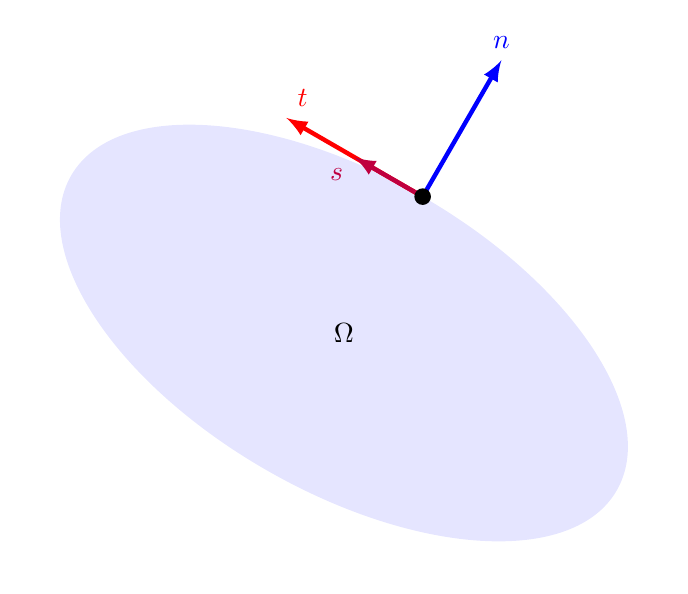
\begin{tikzpicture}
    % \draw[help lines] (0,0) grid (20,10);
    \fill[blue!10] (5,6)  ellipse [x radius=2cm, y radius=4cm, rotate=60];

    % 楕円上の点(x=7 のとき)
    \def\t{0} % t=0 のとき (右端の点) 
    \def\theta{60} % 楕円の回転角
    \def\a{2} % 長半径
    \def\b{4} % 短半径
    \def\cx{5} % 楕円の中心 x 座標
    \def\cy{6} % 楕円の中心 y 座標
    \def\scale{0.5} % ベクトルの縮小率を変更(0.5倍)
    % 点の座標計算
    \pgfmathsetmacro\xval{\cx + \a*cos(\t)*cos(\theta) - \b*sin(\t)*sin(\theta)}
    \pgfmathsetmacro\yval{\cy + \a*cos(\t)*sin(\theta) + \b*sin(\t)*cos(\theta)}
    % 接線ベクトル計算
    \pgfmathsetmacro\Tx{-\a*sin(\t)*cos(\theta) - \b*cos(\t)*sin(\theta)}
    \pgfmathsetmacro\Ty{-\a*sin(\t)*sin(\theta) + \b*cos(\t)*cos(\theta)}
    % 法線ベクトル計算(接線ベクトルを90度回転)
    \pgfmathsetmacro\Nx{\Ty}
    \pgfmathsetmacro\Ny{-\Tx}
    % 接線ベクトルの描画
    \draw[-{latex}, ultra thick, red] (\xval,\yval) -- ++(\scale*\Tx,\scale*\Ty) node[above right] {$\vect{t}$};
    \draw[-{latex}, ultra thick, purple] (\xval,\yval) -- ++(\scale*\scale*\Tx,\scale*\scale*\Ty) node[below left] {$\odif{\vect{s}}$};
    % 法線ベクトルの描画
    \draw[-{latex}, ultra thick, blue] (\xval,\yval) -- ++(\scale*\Nx,\scale*\Ny) node[above] {$\vect{n}$};
    % 点の描画
    \fill[black] (\xval,\yval) circle (3pt);
    \node at (5,6) {$\Omega$};
\end{tikzpicture}
\caption{境界上の点における法線ベクトルの導出}
\end{figure}
ここで,$\vect{t}$は単位接線ベクトル(Unit tangent vector),$\vect{n}$は単位法線ベクトル(Unit normal vector)である.$\vect{t}$は境界上の点の接線ベクトルであり,反時計周りを正とする.$\vect{n}$は$\vect{t}$に対して直角で,境界の外向きを正とする.
ベクトル$\odif{\vect{s}}$は次のように定義できる.
\begin{align}
  \odif{\vect{s}} &= \odif{x}\vect{e}_x + \odif{y}\vect{e}_y\\
  \odif{s} &= \sqrt{\odif{x}^2 + \odif{y}^2}
\end{align}
ここで,$\odif{x}$,$\odif{y}$は境界上の$\odif{\vect{s}}$に対応する変化量であり,$\vect{e}_x$,$\vect{e}_y$はそれぞれ$x$,$y$軸方向の単位ベクトルである.ここで,$\vect{t}$は$\odif{\vect{s}}$をその長さ$\odif{s}$で割ったものである.
\begin{equation}
  \vect{t} = \odv{x}{s}\vect{e}_x + \odv{y}{s}\vect{e}_y
\end{equation}
また,$\vect{n}$は次のように定義される.
\begin{equation}
  \vect{n} = n_x\vect{e}_x + n_y\vect{e}_y
\end{equation}
ここで$\vect{t}$に対して直角であるので,$\vect{t}$と$\vect{n}$の内積は$0$であり,$\vect{t}$と$\vect{n}$の外積は$\vect{e}_z$となる.
\begin{align}
  \label{Eq:tn-dot-product}
  \vect{t}\cdot\vect{n} &= n_x \odv{x}{s} + n_y \odv{y}{s} = 0\\
  \vect{t}\times\vect{n} &= \begin{vmatrix}
    \vect{e}_x & \vect{e}_y & \vect{e}_z\\
    \displaystyle\odv{x}{s} & \displaystyle\odv{y}{s} & 0\\
    n_x & n_y & 0
  \end{vmatrix}=\vect{e}_z\pab{n_x\odv{y}{s} - n_y\odv{x}{s}}=\vect{e}_z\notag\\
  \label{Eq:tn-cross-product}
  &n_x\odv{y}{s} - n_y\odv{x}{s} = 1
\end{align}
\eqref{Eq:tn-dot-product}式と\eqref{Eq:tn-cross-product}式を連立して解くと,最終的に次式を得る.
\begin{equation}
  \vect{n}=\odv{y}{s}\vect{e}_x - \odv{x}{s}\vect{e}_y
\end{equation}
\subsection{一次要素の境界上の積分}
境界上の積分を考える.まず最初にイメージをつかむため,Fig.~\ref{Fig:tri-boundary}に示す三角形要素における境界上の積分を考える.四角形要素においても同様の手法で計算できる.
\begin{figure}
  \centering
  \begin{tikzpicture}
    % \draw[help lines] (0,0) grid (15,12);
    % \node at (0,0) [below left]{$O$};
    \coordinate (p1) at (3,2);
    \coordinate (p2) at (8,4);
    \coordinate (p3) at (5,7);
    \coordinate (G) at ($(p1)!1/3!(p2)!1/3!(p3)$);
    % 縮小率(0.6倍)
    \def\scale{0.6}
    % 内部の三角形の頂点
    \coordinate (p1s) at ($(G)!\scale!(p1)$);
    \coordinate (p2s) at ($(G)!\scale!(p2)$);
    \coordinate (p3s) at ($(G)!\scale!(p3)$);
    \def\lscale{1.18}
    \coordinate (p1o) at ($(G)!\lscale!(p1)$);
    \coordinate (p2o) at ($(G)!\lscale!(p2)$);
    \coordinate (p3o) at ($(G)!\lscale!(p3)$);

    \coordinate[label=below:$q^{(1)}_1$] (p121) at (3.5, 0.75);
    \coordinate[label=below:$q^{(1)}_2$] (p122) at (8.2, 3.5);
    \coordinate[label=above right:$q^{(2)}_1$] (p231) at (8.2, 4.2);
    \coordinate[label=above :$q^{(2)}_2$] (p232) at (5.5, 7.5);
    \coordinate[label=above left:$q^{(3)}_1$] (p311) at (4.5, 7.2);
    \coordinate[label=left:$q^{(3)}_2$] (p312) at (2.0, 2.4);

    \coordinate (p121o) at (3.75, 0);
    \coordinate (p122o) at (8.8,2.0);
    \coordinate (p231o) at (9.0,5.0);
    \coordinate (p232o) at (6.0,8.0);
    \coordinate (p311o) at (3.0,7.75);
    \coordinate (p312o) at (0.86207,2.7552);
    
  
    \draw[fill, color=red!20!white] (p1)--(p2)--(p122)--(p121) -- cycle;
    \draw[fill, color=blue!20!white] (p2)--(p3)--(p232)--(p231) -- cycle;
    \draw[fill, color=green!20!white] (p3)--(p1)--(p312)--(p311) -- cycle;
    \draw[line width=0.4mm] (p1)--(p2)--(p3)--cycle;
      % 内部の縮小三角形の描画
    \draw[-{Latex}] (p1s)--node[midway, above] {$S$}(p2s);
    \draw[-{Latex}] (p2s)--node[midway, right] {$S$}(p3s);
    \draw[-{Latex}] (p3s)--node[midway, right] {$S$}(p1s);
    \draw (p121)--(p122);
    \draw (p231)--(p232);
    \draw (p311)--(p312);
    \foreach \i in {0,1,2,3,4,5,6,7,8,9} {
      \draw[thick, -{Latex}] ($(p1)!\i/9!(p2)$) -- ($(p121)!\i/9!(p122)$);
      \draw[thick, -{Latex}] ($(p2)!\i/9!(p3)$) -- ($(p231)!\i/9!(p232)$);
      \draw[thick, -{Latex}] ($(p3)!\i/9!(p1)$) -- ($(p311)!\i/9!(p312)$);
    }
    \node at (p1o) {$P_1$};
    \node at (p2o) {$P_2$};
    \node at (p3o) {$P_3$};
    \draw[{Latex}-{Latex}] (p121o)--node[midway, below] {$L^{(1)}$}(p122o);
    \draw[{Latex}-{Latex}] (p231o)--node[midway, above right] {$L^{(2)}$}(p232o);
    \draw[{Latex}-{Latex}] (p311o)--node[midway, left] {$L^{(3)}$}(p312o);
  \end{tikzpicture}
  \caption{三角形要素の境界条件}
  \label{Fig:tri-boundary}
\end{figure}\\
境界上の基底関数$\vect{\psi}_\mathrm{b}$は一次元要素と同様に次のように定義される.
\begin{equation}
  \vect{\psi}_\mathrm{b} = \begin{bmatrix}
    1-\dfrac{S}{L}&\dfrac{S}{L}
  \end{bmatrix}
\end{equation}
ここで,$L$は要素境界の長さ,$S$は境界上の局所座標である.よって,$\vect{\psi}_\mathrm{b}$の積の積分は局所座標系に落とし込むことで計算できる.
\begin{equation}
  \int_{\Gamma} \vect{\psi}_\mathrm{b}^\top \vect{\psi}_\mathrm{b} \odif{\Gamma}=\int_{0}^{L}
  \begin{bmatrix}
    \pab{1-\dfrac{S}{L}}\pab{1-\dfrac{S}{L}} & \pab{1-\dfrac{S}{L}}\dfrac{S}{L}\\[2mm]
    \dfrac{S}{L}\pab{1-\dfrac{S}{L}}   & \dfrac{S}{L}\dfrac{S}{L}
  \end{bmatrix}\odif{S}
  =\dfrac{L}{6}
  \begin{bmatrix}
    2 & 1\\
    1 & 2
  \end{bmatrix}
\end{equation}
また,$\vect{\psi}_\mathrm{b}^\top$の積分は次のようになる.
\begin{equation}
  \int_{\Gamma} \vect{\psi}_\mathrm{b}^\top \odif{\Gamma}=\int_{0}^{L}
  \begin{bmatrix}
    1-\dfrac{S}{L}\\[2mm]
    \dfrac{S}{L}
  \end{bmatrix}\odif{S}=\dfrac{L}{2}
  \begin{bmatrix}
    1\\1
  \end{bmatrix}
\end{equation}
ロビン境界を考える場合には少々工夫が必要となる.
\begin{figure}
  \centering
  \begin{tikzpicture}
    \coordinate (p1) at (2,1);
    \coordinate (p2) at (4,6);
    \coordinate[label=below left:$O$] (O) at (0,-1);

    \draw [-{Latex[length=3mm]}] (O) -- (7,-1) node[right] {$x$};
    \draw [-{Latex[length=3mm]}] (O) -- (0,7) node[above] {$y$};
    \draw [very thick] (p1)--(p2);


    \draw [dashed, -{Latex[length=3mm]}] (p1)--++(1.0,0) node[right] {$\vect{q}_x^1$};
    \draw [dashed, -{Latex[length=3mm]}] (p2)--++(0.7,0) node[right] {$\vect{q}_x^2$};
    \draw [dashed, -{Latex[length=3mm]}] (p1)--++(0,-0.8) node[below] {$\vect{q}_y^1$};
    \draw [dashed, -{Latex[length=3mm]}] (p2)--++(0,-1.0) node[below] {$\vect{q}_y^2$};

    \draw [red, -{Latex[length=3mm]}] (p1)--++(1.137931034482759, -0.4551724137931035) node[below right] {$\vect{q}_1\cdot\vect{n}$};
    \draw [red, -{Latex[length=3mm]}] (p2)--++(0.9482758620689657, -0.37931034482758624) node[below right] {$\vect{q}_2\cdot\vect{n}$};

    \fill [black] (p1) circle (2.2pt) node[below left] {$P_1$};
    \fill [black] (p2) circle (2.2pt) node[above right] {$P_2$};
  \end{tikzpicture}
\end{figure}\\
境界上の節点には,直交座標系における熱フラックス$\vect{q}_x$,$\vect{q}_y$が与えられている.これを局所座標系に変換するために,$\vect{q}_x$,$\vect{q}_y$を$\vect{n}$に射影する.
\begin{subequations}
  \begin{align}
    \vect{Q}_\mathrm{Cn,1}&=\vect{q}_1\cdot\vect{n}=\vect{q}_x^1n_x + \vect{q}_y^1n_y\\
    \vect{Q}_\mathrm{Cn,2}&=\vect{q}_2\cdot\vect{n}=\vect{q}_x^2n_x + \vect{q}_y^2n_y
  \end{align}
\end{subequations}
この射影したベクトル$\vect{Q}_\mathrm{Cn}$を用いて,ロビン境界の節点における積分を計算する.
\subsection{二次要素の境界上の積分}

\subsection{Gauss-Legendre積分}
\begin{NoteBox}{Gauss-Legendre積分の二次元への拡張}{Integral-Gauss-Legendre-2D}
  \begin{equation}
    \label{Eq:Gauss-Legendre-2D}
    \int_{-1}^{+1}\int_{-1}^{+1} f\pab{\xi, \eta}\odif{\xi}\odif{\eta} \approx \sum_{i=1}^{N_\mathrm{sample}}\sum_{j=1}^{N_\mathrm{sample}}w_i w_j f\pab{\xi_i, \eta_j}
  \end{equation}
  \small
  $N_\mathrm{sample}$:サンプル点の数,$w_i$:重み,$\xi_i$,$\eta_i$:サンプル点
\end{NoteBox}
\eqref{Eq:Gauss-Legendre-2D}式を用いたときの積分の概念図を示す.このとき,サンプル点は2点とする.
\begin{figure}[H]
  \centering
  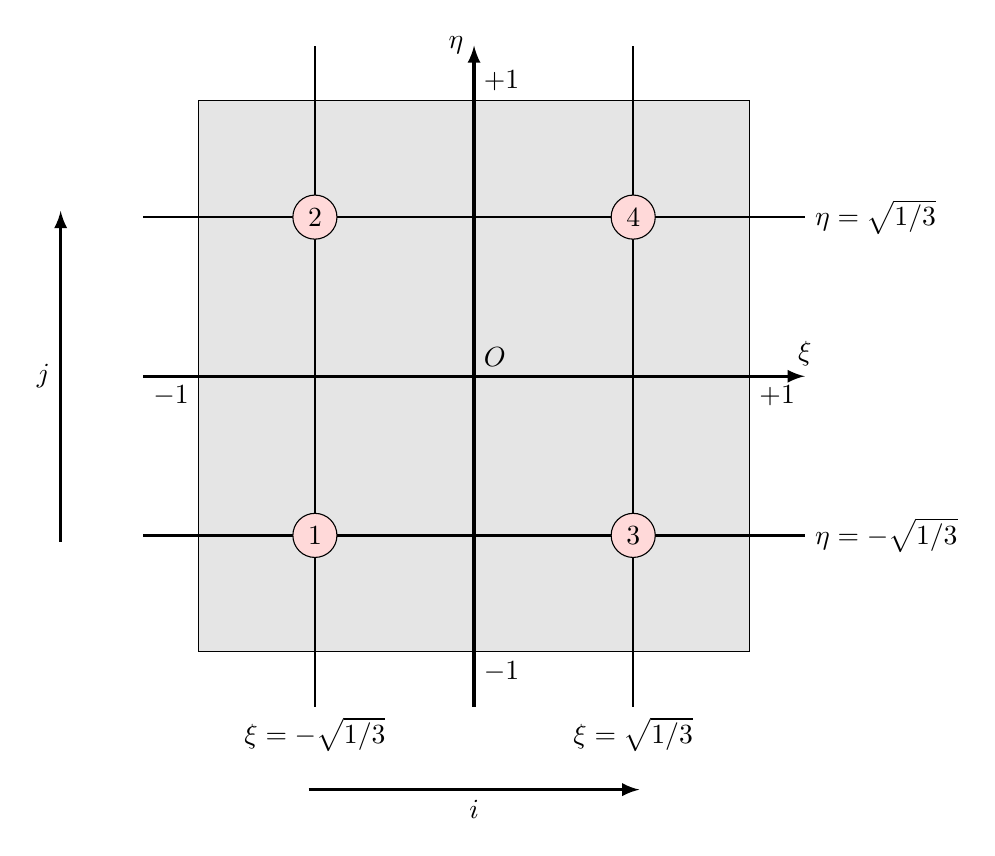
\begin{tikzpicture}[scale=3.5]
    \coordinate (p1) at (-1,-1);
    \coordinate (p2) at (1,-1);
    \coordinate (p3) at (1,1);
    \coordinate (p4) at (-1,1);
    \coordinate (S1) at (-0.57735,-0.57735);
    \coordinate (S2) at (-0.57735, 0.57735);
    \coordinate (S3) at ( 0.57735,-0.57735);
    \coordinate (S4) at ( 0.57735, 0.57735);

    \draw[fill=black!10!white] (p1)--node[midway, below right]{$-1$}(p2)--node[midway, below right]{$+1$}(p3)--node[midway, above right]{$+1$}(p4)--cycle node[midway, below left]{$-1$};
    \coordinate[label=above right:$O$] (O) at (0,0);
    %axis
    \draw[-{latex}, line width=0.4mm] (-1.2,0) -- (1.2,0) node[above]{$\xi$};
    \draw[-{latex}, line width=0.4mm] (0,-1.2) -- (0,1.2) node[left]{$\eta$};

    \draw[-{latex}, line width=0.4mm] (-0.6,-1.5) --node[midway, below]{$i$} (0.6,-1.5);
    \draw[-{latex}, line width=0.4mm] (-1.5,-0.6) --node[midway, left]{$j$} (-1.5,0.6);

    \draw[-, line width=0.3mm] (-1.2, 0.57735) -- (1.2, 0.57735) node[right]{$\eta= \sqrt{1/3}$};
    \draw[-, line width=0.3mm] (-1.2,-0.57735) -- (1.2,-0.57735) node[right]{$\eta=-\sqrt{1/3}$};
    \draw[-, line width=0.3mm] (-0.57735,-1.2) node[below]{$\xi=-\sqrt{1/3}$} -- (-0.57735,1.2);
    \draw[-, line width=0.3mm] ( 0.57735,-1.2) node[below]{$\xi= \sqrt{1/3}$} -- ( 0.57735,1.2);

    \foreach \i in {1,2,3,4} {
      \draw[fill=pink!60!white] (S\i) node {\i} circle[radius=0.08];
    }
  \end{tikzpicture}
  \caption{Gauss-Legendre積分のサンプル点を2点とした場合の積分の概念図}
\end{figure}
サンプル点は増やすことができる.サンプル点数に応じた,重みとサンプル点を表に示す.
\begin{longtable}{ccc}
  % \centering
  \caption{Gauss-Legendre積分のサンプル点数に応じた重みとサンプル点}\\
  % \begin{tabular}
    \hline
    サンプル点数:$N_\mathrm{sample}$ & サンプル点:$\xi_i$,$\eta_i$ & 重み:$w_i$,$w_j$\\
    \hline
    $1$ & $0$ & $2$\\
    \hline
    &&\\[-6mm]
    $2$ & $\pm\sqrt{\dfrac{1}{3}}$ & $1$\\[4mm]
    \hline
    &&\\[-6mm]
    $3$ & $0$ & $\dfrac{8}{9}$\\[4mm]
     & $\pm\sqrt{\dfrac{3}{5}}$ & $\dfrac{5}{9}$\\[4mm]
    \hline
    &&\\[-6mm]
    $4$ & $\pm\sqrt{\dfrac{3}{7}-\dfrac{2}{7}\sqrt{\dfrac{6}{5}}}$ & $\dfrac{18+\sqrt{30}}{36}$\\[4mm]
     & $\pm\sqrt{\dfrac{3}{7}+\dfrac{2}{7}\sqrt{\dfrac{6}{5}}}$ & $\dfrac{18-\sqrt{30}}{36}$\\[4mm]
    \hline
    &&\\[-6mm]
    $5$ & $0$ & $\dfrac{128}{225}$\\[4mm]
     & $\pm\dfrac{1}{3}\sqrt{5-2\sqrt{\dfrac{10}{7}}}$ & $\dfrac{322+13\sqrt{70}}{900}$\\[4mm]
     & $\pm\dfrac{1}{3}\sqrt{5+2\sqrt{\dfrac{10}{7}}}$ & $\dfrac{322-13\sqrt{70}}{900}$\\[4mm]
    \hline
  % \end{tabular}
\end{longtable}

何個か例題を解いて,精度を見てみることとする.

\begin{ExampleBox}{ガウス求積法}{GL-Integral-Example}
  Gauss-Legendre積分を用いて次の積分を求め,解析解と比較せよ.
  \begin{enumerate}[label=(\arabic*)]
    \item
    \begin{equation*}
      \int_{-1}^{+1}\int_{-1}^{+1} \pab{x^2 + y^2}\odif{x}\odif{y}
    \end{equation*}
    \item
    \begin{equation*}
      \int_{-1}^{+1}\int_{-1}^{+1} \pab{x^3 + y^3}\odif{x}\odif{y}
    \end{equation*}
    \item
    \begin{equation*}
      \int_{-1}^{+1}\int_{-1}^{+1} \exp\pab{-x^2 - y^2}\odif{x}\odif{y}
    \end{equation*}
    \item
    \begin{equation*}
      \int_{-1}^{+1}\int_{-1}^{+1} \pab{\sin x \cos y}\odif{x}\odif{y}
    \end{equation*}
  \end{enumerate}
\end{ExampleBox}
例題\ref{Exa:GL-Integral-Example}の解答を示す.

\begin{longtable}[c]{cS[table-format=1.8e-2] S[table-format=1.8e-2] S[table-format=1.8e-2] c}
  \caption{数値計算結果と解析解} \label{tab:results} \\

  \toprule
  & {$N_\mathrm{sample}$} & {結果} & {誤差} & {解析解} \\
  \midrule
  \endfirsthead

  \multicolumn{5}{c}%
  {{\bfseries 表 \thetable\  続き}} \\
  \toprule
  & {$N_\mathrm{sample}$} & {結果} & {誤差} & {解析解} \\
  \midrule
  \endhead

  \midrule
  \multicolumn{5}{r}{{続く}} \\
  \endfoot

  \bottomrule
  \endlastfoot

  \multirow{5}{*}{(1)} 
    & 1 & \SI{0.00000000E+00}{} & \SI{2.66666667E+00}{} & \multirow{5}{*}{\(\dfrac{8}{3}\)} \\
    & 2 & \SI{2.66666667E+00}{} & \SI{0.00000000E+00}{} &  \\
    & 3 & \SI{2.66666667E+00}{} & \SI{4.44089210E-16}{} &  \\
    & 4 & \SI{2.66666667E+00}{} & \SI{4.44089210E-16}{} &  \\
    & 5 & \SI{2.66666667E+00}{} & \SI{4.44089210E-16}{} &  \\
  \midrule
  \multirow{5}{*}{(2)} 
    & 1 & \SI{0.00000000E+00}{} & \SI{0.00000000E+00}{} & \multirow{5}{*}{\(0\)} \\
    & 2 & \SI{0.00000000E+00}{} & \SI{0.00000000E+00}{} &  \\
    & 3 & \SI{-5.55111512E-17}{} & \SI{5.55111512E-17}{} &  \\
    & 4 & \SI{2.77555756E-17}{} & \SI{2.77555756E-17}{} &  \\
    & 5 & \SI{1.38777878E-17}{} & \SI{1.38777878E-17}{} &  \\
  \midrule
  \multirow{5}{*}{(3)} 
    & 1 & \SI{4.00000000E+00}{} & \SI{1.76901486E+00}{} & \multirow{5}{*}{\(\pi\,\mathrm{erf}(1)^2\)} \\
    & 2 & \SI{2.05366848E+00}{} & \SI{1.77316665E-01}{} &  \\
    & 3 & \SI{2.24604053E+00}{} & \SI{1.50553890E-02}{} &  \\
    & 4 & \SI{2.23004829E+00}{} & \SI{9.36846798E-04}{} &  \\
    & 5 & \SI{2.23103191E+00}{} & \SI{4.67666046E-05}{} &  \\
  \midrule
  \multirow{5}{*}{(4)} 
    & 1 & \SI{0.00000000E+00}{} & \SI{0.00000000E+00}{} & \multirow{5}{*}{\(0\)} \\
    & 2 & \SI{0.00000000E+00}{} & \SI{0.00000000E+00}{} &  \\
    & 3 & \SI{-2.77555756E-17}{} & \SI{2.77555756E-17}{} &  \\
    & 4 & \SI{1.38777878E-17}{} & \SI{1.38777878E-17}{} &  \\
    & 5 & \SI{0.00000000E+00}{} & \SI{0.00000000E+00}{} &  \\
\end{longtable}

\begin{figure}[H]
  \centering
  \subfigure[$f\pab{x,y}=x^2 + y^2$]{\includegraphics[width=0.45\textwidth]{Gauss_f1.png}}
  \subfigure[$f\pab{x,y}=x^3 + y^3$]{\includegraphics[width=0.45\textwidth]{Gauss_f2.png}} \\
  \subfigure[$f\pab{x,y}=\exp\pab{-x^2 - y^2}$]{\includegraphics[width=0.45\textwidth]{Gauss_f3.png}}
  \subfigure[$f\pab{x,y}=\sin x \cos y$]{\includegraphics[width=0.45\textwidth]{Gauss_f4.png}}
  \caption{例題1の関数の概形}
\end{figure}
ただし,基底関数の積分においては基本的には要素が持っている次数+1のサンプル点数を用いることが多い.
また,必ずしもGauss-Legendre積分による積分が精度が保証されているわけではないので注意されたい.要素次元を増やすことよりも,サンプル点の座標をうまく調整することで精度を向上させることができる.例えば,2点での積分を行う場合には,サンプル点を$\xi_i=\pm 0.8165$とすることで,精度を向上させることができる.
\subsection{可変時間ステップおよび可変次数における後退差分法}
\label{Sec:BDF}
後退差分法(Backward Differentiation Formula, BDF)は,時間積分において,過去の値を用いて現在の値を求める方法である.BDFは,特に支配方程式の系が硬い問題において有効であり,数値的な安定性が高い特徴を持つ.7次以上は零点安定性がなくなるので考える必要はなく,6次までのBDFを考えることとする.
時間微分項 $\pdv{\vect{T}}/{t}$ を近似するため,いくつかの過去の時点 $(t_i, \vect{T}^i)$ を通るラグランジュ補間多項式 $P(t)$ を構築し,その現在時刻 $t_{n+1}$ での微分 $P'(t_{n+1})$ を用いる.
一般にLagrange補間多項式は,Lagrange基底関数 $l_i(x)$
\begin{align}
  l_i(x) = \prod_{\substack{j=0\leq j \leq i \\[0.2mm] j \neq i}}\frac{x - x_j}{x_i - x_j}
\end{align}
と補間対象となる変数$y_i$との線形結合として与えられる.
\begin{equation}
  \label{eq:bdf_lagrange}
  L\pab{x}\coloneq\sum_{i=0}^{j} y_i l_i \pab{x}
\end{equation}
計算を簡略化するため,局所的な時間座標 $\tau = t - t_{n+1}$ を導入する.この座標系では,現在時刻は $\tau=0$ となる.ただし,1次のBDFは単純な後退差分であるため,2次以上のBDFについて考える.本節では特に2次について詳述するとともに,6次までのBDFはそれまでと同様に導出できるため,その結果を示すだけとする.本章ではk-次数のBDFをBDF-kと表記する.

\subsubsection{BDF-2における導出}
3つの点 $(t_{n+1}, \vect{T}^{n+1})$,$(t_n, \vect{T}^n)$,$(t_{n-1}, \vect{T}^{n-1})$ を通る2次のラグランジュ補間多項式 $P(\tau)$ を考える.各点は局所座標で $(\tau_0, \vect{T}^{n+1}), (\tau_1, \vect{T}^n), (\tau_2, \vect{T}^{n-1})$ と表せる.
\begin{subequations}
  \label{eq:bdf2_lagrange_time}
  \begin{align}
    \tau_0 & = t_{n+1} - t_{n+1} = 0                              \\
    \tau_1 & = t_n - t_{n+1} = -\Delta t_n                        \\
    \tau_2 & = t_{n-1} - t_{n+1} = -(\Delta t_n + \Delta t_{n-1})
  \end{align}
\end{subequations}
ここで$P\pab{\tau}$が$k=2$の時のLagrange補間多項式であるとすると,\eqref{eq:bdf_lagrange}式より
\begin{align}
  P\pab{\tau} = \vect{T}^{n+1} l_0(\tau) + \vect{T}^n l_1(\tau) + \vect{T}^{n-1} l_2(\tau)
\end{align}
ここで,各基底関数は次のように定義される.
\begin{subequations}
  \label{eq:bdf2_lagrange_basis}
  \begin{align}
    l_0\pab{\tau} = \frac{\tau-\tau_1}{\tau_0-\tau_1} \frac{\tau-\tau_2}{\tau_0-\tau_2} \\[1mm]
    l_1\pab{\tau} = \frac{\tau-\tau_0}{\tau_1-\tau_0} \frac{\tau-\tau_2}{\tau_1-\tau_2} \\[1mm]
    l_2\pab{\tau} = \frac{\tau-\tau_0}{\tau_2-\tau_0} \frac{\tau-\tau_1}{\tau_2-\tau_1}
  \end{align}
\end{subequations}
ここで各基底関数の微分は\eqref{eq:bdf2_lagrange_basis}式より
\begin{subequations}
  \label{eq:bdf2_lagrange_basis_diff}
  \begin{align}
    l'_0\pab{\tau} & = \frac{\tau-\tau_2}{\pab{\tau_0-\tau_1}\pab{\tau_0-\tau_2}} + \frac{\tau-\tau_1}{\pab{\tau_0-\tau_1}\pab{\tau_0-\tau_2}} = \frac{2\tau - \tau_1 - \tau_2}{\pab{\tau_0-\tau_1}\pab{\tau_0-\tau_2}} \\[1mm]
    l'_1\pab{\tau} & = \frac{\tau-\tau_2}{\pab{\tau_1-\tau_0}\pab{\tau_1-\tau_2}} + \frac{\tau-\tau_0}{\pab{\tau_1-\tau_0}\pab{\tau_1-\tau_2}} = \frac{2\tau - \tau_0 - \tau_2}{\pab{\tau_1-\tau_0}\pab{\tau_1-\tau_2}} \\[1mm]
    l'_2\pab{\tau} & = \frac{\tau-\tau_1}{\pab{\tau_2-\tau_0}\pab{\tau_2-\tau_1}} + \frac{\tau-\tau_0}{\pab{\tau_2-\tau_0}\pab{\tau_2-\tau_1}} = \frac{2\tau - \tau_0 - \tau_1}{\pab{\tau_2-\tau_0}\pab{\tau_2-\tau_1}}
  \end{align}
\end{subequations}
$P\pab{\tau}$ の $\tau=0$ における微分は,
\begin{equation}
  P'\pab{0} = \vect{T}^{n+1}l'_0(0) + \vect{T}^n l'_1(0) + \vect{T}^{n-1}l'_2(0)
\end{equation}
これに\eqref{eq:bdf2_lagrange_basis_diff}および$\tau_1, \tau_2$ を代入し,時間ステップ比 $\rho_1 = \Delta t_n / \Delta t_{n-1}$ を用いて整理すると,
\begin{subequations}
  \begin{align}
    l'_0\pab{0} & = -\frac{\tau_1 + \tau_2}{\tau_1 \tau_2} = \frac{2\Delta t_n + \Delta t_{n-1}}{\Delta t_n \pab{\Delta t_n + \Delta t_{n-1}}} = \frac{2\rho_1 + 1}{\rho_1 + 1}\frac{1}{\Delta t_n} \\[2mm]
    l'_1\pab{0} & = -\frac{\tau_2}{\tau_1 \pab{\tau_1 - \tau_2}} = -\frac{\Delta t_n + \Delta t_{n-1}}{\Delta t_n \Delta t_{n-1}} = -\pab{\rho + 1}\frac{1}{\Delta t_n}                             \\[2mm]
    l'_2\pab{0} & = -\frac{\tau_1}{\tau_2 \pab{\tau_2 - \tau_1}} = \frac{\Delta t_n}{\pab{\Delta t_n + \Delta t_{n-1}}\Delta t_{n-1} } = \frac{\rho_1^2}{\rho_1 + 1}\frac{1}{\Delta t_n}
  \end{align}
\end{subequations}
よって,時間微分の近似式は,
\begin{equation}
  \label{eq:bdf2_approx}
  \pdv{\vect{T}}{t} \bigg|_{t_{n+1}} \approx \frac{1}{\Delta t_n} \bab{\frac{2\rho_1 + 1}{\rho_1 + 1}\vect{T}^{n+1} - \pab{\rho_1 + 1} \vect{T}^n + \frac{\rho_1^2}{\rho_1 + 1} \vect{T}^{n-1}}
\end{equation}

\subsubsection{BDF-$k$における導出結果}
BDF-$k$においては,$k$個の過去の時点を用いて微分を近似する.
一般に,時間ステップをくくりだすことで,$k$次のBDFは次のように定義される.
\begin{equation}
  \label{eq:bdf_k_approx}
  \pdv{\vect{T}}{t} \bigg|_{t_{n+1}} \approx \frac{1}{\Delta t_n} \sum_{i=0}^{k} l'_i\pab{0} \vect{T}^{n+1-i}
\end{equation}
ここで,$l_i$はBDF-$k$における係数であり,BDF-$k$の係数はCode Snippet\ref{prog:bdf_coeffs_final}を用いて求めることができる.
% ここで,$l_i$はBDF-kにおける係数であり,BDF-kの係数は次のように与えられる.ただし,$\rho_i=\Delta t_{n+1-i} / \Delta t_{n-i}$とする.ここで式を簡略化するために,$\displaystyle r_{ki}\coloneq\prod_{j=k}^{i} \rho_j$と定義する.
% \begin{itemize}
%   \item $k=3$のとき
%         \begin{subequations}
%           \begin{align}
%             l'_0\pab{0} & = \frac{3 r_{12} \rho_2 + 4 r_{12} + 2 \rho_1 + \rho_2 + 1}{\pab{\rho_1 + 1}\pab{r_{12} + \rho_2 + 1}} \\[2mm]
%             l'_1\pab{0} & = -\frac{\pab{\rho_1 + 1}\pab{r_{12} + \rho_2 + 1}}{\rho_2 + 1}                                        \\[2mm]
%             l'_2\pab{0} & = \frac{\rho_1^2 \pab{r_{12} + \rho_2 + 1}}{\rho_1 + 1}                                                \\[2mm]
%             l'_3\pab{0} & = -\frac{r_{12}^2 \rho_2\pab{\rho_1 + 1}}{\pab{\rho_2 + 1}\pab{r_{12} + \rho_2 + 1}}
%           \end{align}
%         \end{subequations}
%   \item $k=4$のとき
%         \begin{subequations}
%           \begin{align}
%             l'_0(0) & = \frac{1}{(\rho_1 + 1)(r_{12} + \rho_2 + 1)(r_{13} + r_{23} + \rho_3 + 1)}\notag                                             \\[1mm]
%                     & \quad \bigl(4 \rho_1 r_{12} r_{13} + 9 r_{12} r_{13} + 6 \rho_1 r_{13} + 3 \rho_1 r_{12} + 6 \rho_2 r_{13} + 8 r_{13}  \notag \\[1mm]
%                     & \quad + 4 r_{12} + 2 r_{31}  + \rho_2 r_{23} + 2 \rho_{23} + 2 \rho_1 + \rho_2 + \rho_3 + 1\bigr)                             \\[2mm]
%             l'_1(0) & = -\frac{
%               (\rho_1 + 1)(r_{12} + \rho_2 + 1)(r_{13} + r_{23} + \rho_3 + 1)
%             }{
%               (\rho_2 + r_{23} + \rho_3 + 1)
%             }                                                                                                                                       \\[2mm]
%             l'_2(0) & = \frac{
%               \rho_1^2 (r_{12} + \rho_2 + 1)(r_{13} + r_{23} + \rho_3 + 1)
%             }{
%               (\rho_1 + 1)(\rho_3 + 1)
%             }                                                                                                                                       \\[2mm]
%             l'_3(0) & = -\frac{
%               \rho_2 r_{12}^2 (\rho_1 + 1)(r_{13} + r_{23} + \rho_3 + 1)
%             }{
%               (\rho_2 + 1)(r_{12} + \rho_2 + 1)
%             }                                                                                                                                       \\[2mm]
%             l'_4(0) & = \frac{
%               \rho_3 r_{13}^2 r_{23} (\rho_1 + 1)(r_{12} + \rho_2 + 1)
%             }{
%               (\rho_3 + r_{23} + \rho_3 + 1)(r_{13} + r_{23} + \rho_3 + 1)
%             }
%           \end{align}
%         \end{subequations}
%   \item $k=5$のとき
%         \begin{subequations}
%           \begin{align}
%             l'_0(0) & = \frac{1}{
%               \pab{\rho_1 + 1}
%               \pab{r_{12} + \rho_2 + 1}
%               \pab{r_{13} + r_{23} + \rho_3 + 1}
%               \pab{r_{14} + r_{24} + r_{34} + \rho_4 + 1}}
%             \notag                                                                                                                      \\
%                     & \quad \bigl(
%             5 \rho_1 r_{14} r_{13} r_{12}
%             + 16 r_{14} r_{13} r_{12}
%             + 12 \rho_1 r_{13} r_{12}
%             + 8 \rho_1 r_{14} r_{12}
%             + 4 \rho_1 r_{13} r_{12}
%             \notag                                                                                                                      \\
%                     & \quad
%             + 18 \rho_2 r_{14} r_{13}
%             + 27 r_{14} r_{13}
%             + 18 r_{14} r_{12}
%             + 9 r_{13} r_{12}
%             + 9 \rho_1 \rho_3 r_{14}
%             + 12 \rho_1 r_{14}
%             + 6 \rho_1 r_{13}
%             \notag                                                                                                                      \\
%                     & \quad
%             + 3 \rho_1 r_{42}
%             + 3 \rho_1 r_{12}
%             + 8 \rho_2 r_{14} r_{23}
%             + 18 r_{14} r_{23}
%             + 12 \rho_2 r_{14}
%             + 6 \rho_2 r_{13}
%             + 12 \rho_3 r_{14}
%             \notag                                                                                                                      \\
%                     & \quad
%             + 16 r_{14}
%             + 8 r_{13}
%             + 4 r_{42}
%             + 4 r_{12}
%             + 2 \rho_1 \rho_3 r_{34}
%             + 4 \rho_1 r_{34}
%             + 2 \rho_1 \rho_3
%             + 2 r_{41}
%             + 2 \rho_1
%             \notag                                                                                                                      \\
%                     & \quad
%             + \rho_2 r_{24} r_{34}
%             + 3 r_{24} r_{34}
%             + 2 \rho_2 r_{24}
%             + \rho_2 r_{23}
%             + 3 \rho_3 r_{24}
%             + 4 r_{24}
%             + 2 r_{23}
%             + \rho_2 \rho_4
%             + \rho_2
%             \notag                                                                                                                      \\
%                     & \quad
%             + \rho_3 r_{34}
%             + 2 r_{34}
%             + \rho_3
%             + \rho_4
%             + 1
%             \bigr)
%             \\[2mm]
%             %
%             l'_1(0) & = -\frac{(\rho_1 + 1)(r_{12} + \rho_2 + 1)(r_{13} + r_{23} + \rho_3 + 1)(r_{14} + r_{24} + r_{34} + \rho_4 + 1)}{
%               (\rho_2 + 1)(r_{23} + \rho_3 + 1)(r_{24} + r_{34} + \rho_4 + 1)}
%             \\[2mm]
%             %
%             l'_2(0) & = \frac{\rho_1^2 (r_{12} + \rho_2 + 1)(r_{13} + r_{23} + \rho_3 + 1)(r_{14} + r_{24} + r_{34} + \rho_4 + 1)}{
%               (\rho_1 + 1)(\rho_3 + 1)(r_{34} + \rho_4 + 1)}
%             \\[2mm]
%             %
%             l'_3(0) & = -\frac{r_{12}^2 \rho_2 (\rho_1 + 1)(r_{13} + r_{23} + \rho_3 + 1)(r_{14} + r_{24} + r_{34} + \rho_4 + 1)}{
%               (\rho_2 + 1)(\rho_4 + 1)(r_{12} + \rho_2 + 1)}
%             \\[2mm]
%             %
%             l'_4(0) & = \frac{r_{13}^2 r_{23} \rho_3 (\rho_1 + 1)(r_{12} + \rho_2 + 1)(r_{14} + r_{24} + r_{34} + \rho_4 + 1)}{
%               (\rho_3 + 1)(r_{23} + \rho_3 + 1)(r_{13} + r_{23} + \rho_3 + 1)}
%             \\[2mm]
%             %
%             l'_5(0) & = -\frac{r_{14}^2 r_{24} r_{34} \rho_4 (\rho_1 + 1)(r_{12} + \rho_2 + 1)(r_{13} + r_{23} + \rho_3 + 1)}{
%               (\rho_4 + 1)(r_{34} + \rho_4 + 1)(r_{24} + r_{34} + \rho_4 + 1)(r_{14} + r_{24} + r_{34} + \rho_4 + 1)}
%           \end{align}
%         \end{subequations}
%   \item $k=6$のとき
%         \begin{subequations}
%           \begin{align}
%             l'_0(0)   & = \frac{1}{
%               \pab{\rho_1 + 1}
%               \pab{r_{12} + \rho_2 + 1}
%               \pab{r_{13} + r_{23} + \rho_3 + 1}
%               \pab{r_{14} + r_{24} + r_{34} + \rho_4 + 1}
%               \pab{r_{15} + r_{25} + r_{35} + r_{45} + \rho_5 + 1}}
%             \notag                                                                                                                                                                                                                  \\[2mm]
%                       & \quad \bigl(
%             6 \rho_{1} r_{15} r_{14} r_{13} r_{12}^{2}
%             + 25 r_{15} r_{14} r_{13} r_{12}
%             + 20 \rho_{1} r_{15} r_{14} r_{13}
%             + 15 \rho_{1} r_{15} r_{14} r_{12}
%             + 10 \rho_{1} r_{15} r_{13} r_{12} \notag                                                                                                                                                                               \\[1mm]
%                       & \quad + 5 \rho_{1} r_{14} r_{13} r_{12}
%             + 40 \rho_{2} r_{15} r_{14} r_{13}
%             + 64 r_{15} r_{14} r_{13}
%             + 48 r_{15} r_{14} r_{12}
%             + 32 r_{15} r_{13} r_{12}
%             + 16 r_{14} r_{13} r_{12} \notag                                                                                                                                                                                        \\[1mm]
%                       & \quad + 24 \rho_{1}  \rho_{3} r_{15} r_{14}
%             + 36 \rho_{1} r_{15} r_{14}
%             + 24 \rho_{1} r_{15} r_{13}
%             + 12 \rho_{1} r_{14} r_{13}
%             + 12 \rho_{4} r_{15} r_{12}
%             + 16 \rho_{1} r_{15} r_{12} \notag                                                                                                                                                                                      \\[1mm]
%                       & \quad + 8 \rho_{1} r_{14} r_{12}
%             + 4 \rho_{1} \rho_{5} r_{13} r_{12}
%             + 4 \rho_{1} r_{13} r_{12}
%             + 30 \rho_{2} r_{15} r_{14} r_{23}
%             + 72 r_{15} r_{14} r_{23}
%             + 54 \rho_{2} r_{15} r_{14} \notag                                                                                                                                                                                      \\[1mm]
%                       & \quad + 36 \rho_{2} r_{15} r_{13}
%             + 18 \rho_{2} r_{14} r_{13}
%             + 54 \rho_{3} r_{15} r_{14}
%             + 81 r_{15} r_{14}
%             + 54 r_{15} r_{13}
%             + 27 r_{14} r_{13}
%             + 27 \rho_{4} r_{15} r_{12} \notag                                                                                                                                                                                      \\[1mm]
%                       & \quad + 36 r_{15} r_{12}
%             + 18 r_{14} r_{12}
%             + 9 r_{53} r_{12}
%             + 9 r_{13} r_{12}
%             + 12 \rho_{1} \rho_{3} r_{15} r_{34}
%             + 27 \rho_{1} r_{15} r_{34}
%             + 18 \rho_{1} \rho_{3} r_{15} \notag                                                                                                                                                                                    \\[1mm]
%                       & \quad + 9 \rho_{1} \rho_{3} r_{14}
%             + 18 \rho_{1} \rho_{4} r_{15}
%             + 24 \rho_{1} r_{15}
%             + 12 \rho_{1} r_{14}
%             + 6 \rho_{1} \rho_{5} r_{13}
%             + 6 \rho_{1} r_{13}
%             + 3 \rho_{1} \rho_{4} r_{42}
%             + 6 \rho_{1} r_{42} \notag                                                                                                                                                                                              \\[1mm]
%                       & \quad + 3 \rho_{1}\rho_{4} r_{12}
%             + 3 \rho_{1} r_{52}
%             + 3 \rho_{1} r_{12}
%             + 10 \rho_{2} r_{15} r_{24} r_{23}
%             + 32 r_{15} r_{24} r_{23}
%             + 24 \rho_{2} r_{15} r_{24}
%             + 16 \rho_{2} r_{15} r_{23} \notag                                                                                                                                                                                      \\[1mm]
%                       & \quad + 8 \rho_{2} r_{14} r_{23}
%             + 36 \rho_{3} r_{15} r_{24}
%             + 54 r_{15} r_{24}
%             + 36 r_{15} r_{23}
%             + 18 r_{14} r_{23}
%             + 18 \rho_{2} \rho_{4} r_{15} r_{24}
%             + 24 \rho_{2} r_{15}  \notag                                                                                                                                                                                            \\[1mm]
%                       & \quad + 12 \rho_{2} r_{14}
%             + 6 \rho_{2} r_{53}
%             + 6 \rho_{2} r_{13}
%             + 16 \rho_{3} r_{15} r_{34}
%             + 36 r_{15} r_{34}
%             + 24 \rho_{3} r_{15}
%             + 12 \rho_{3} r_{14}
%             + 24 \rho_{4} r_{15} \notag                                                                                                                                                                                             \\[1mm]
%                       & \quad + 32 r_{15}
%             + 16 r_{14}
%             + 8 r_{53}
%             + 8 r_{13}
%             + 4 \rho_{4} r_{42}
%             + 8 r_{42}
%             + 4 \rho_{4} r_{12}
%             + 4 r_{52}
%             + 4 r_{12}
%             + 2 \rho_{3} r_{31} r_{34} \notag                                                                                                                                                                                       \\[1mm]
%                       & \quad + 6 r_{31} r_{34}
%             + 4 \rho_{3} r_{31}
%             + 2 \rho_{1} \rho_{3} r_{34}
%             + 6 \rho_{4} r_{31}
%             + 8 r_{31}
%             + 4 \rho_{1} r_{34}
%             + 2 \rho_{1} \rho_{3} \rho_{5}
%             + 2 \rho_{1} \rho_{3}
%             + 2 \rho_{4} r_{41} \notag                                                                                                                                                                                              \\[1mm]
%                       & \quad + 4 \rho_{1} r_{45}
%             + 2 \rho_{1} \rho_{4}
%             + 2 \rho_{1} \rho_{5}
%             + 2 \rho_{1}
%             + \rho_{2} \rho_{4} r_{23}^3 r_{45}
%             + 4 \rho_{4} r_{23}^3 r_{45}
%             + 3 \rho_{2} \rho_{4} r_{23}^2 r_{45}
%             + 2 \rho_{2} r_{23}^2 r_{45}  \notag                                                                                                                                                                                    \\[1mm]
%                       & \quad + \rho_{2} r_{24} r_{23}
%             + 6 \rho_{3} r_{25} r_{24}
%             + 9 r_{25} r_{24}
%             + 6 r_{25} r_{23}
%             + 3 r_{24} r_{23}
%             + 3 \rho_{2} \rho_{4} r_{25}
%             + 4 \rho_{2} r_{25}
%             + 2 \rho_{2} r_{24} \notag                                                                                                                                                                                              \\[1mm]
%                       & \quad + \rho_{2} \rho_{5} r_{23}
%             + \rho_{2} r_{23}
%             + 4 \rho_{3} r_{25} r_{34}
%             + 9 r_{25} r_{34}
%             + 6 \rho_{3} r_{25}
%             + 3 \rho_{3} r_{24}
%             + 6 \rho_{4} r_{25}
%             + 8  r_{25}
%             + 4  r_{24}  \notag                                                                                                                                                                                                     \\[1mm]
%                       & \quad + 2 \rho_{5} r_{23}
%             + 2 r_{23}
%             + \rho_{4} r_{45}
%             + 2 \rho_{2} r_{45}
%             + \rho_{2} \rho_{4}
%             + \rho_{2} \rho_{5}
%             + \rho_{2}
%             + \rho_{3} r_{35} r_{34}
%             + 3 r_{35} r_{34}
%             + 2 \rho_{3} r_{35} \notag                                                                                                                                                                                              \\[1mm]
%                       & \quad + \rho_{3} r_{34}
%             + 3 \rho_{4} r_{35}
%             + 4 r_{35}
%             + 2 r_{34}
%             + \rho_{3} \rho_{5}
%             + \rho_{3}
%             + \rho_{4} r_{45}
%             + 2 r_{45}
%             + \rho_{4}
%             + \rho_{5}
%             + 1
%             \bigr)                                                                                                                                                                                                                  \\[2mm]
%             l'_{1}(0) & = - \frac{1}{\pab{\rho_{2} + 1} \pab{r_{23} + \rho_{3} + 1} \pab{r_{24} + r_{34} + \rho_{4} + 1} \pab{r_{25} + r_{35} + r_{45} + \rho_{5} + 1}} \notag                                                      \\[1mm]
%                       & \qquad \pab{\rho_{1} + 1} \pab{r_{12} + \rho_{2} + 1}
%             \pab{r_{13} + r_{23} + \rho_{3} + 1} \notag                                                                                                                                                                             \\[1mm]
%                       & \qquad \pab{r_{14} + r_{24} + r_{34} + \rho_{4} + 1}
%             \pab{r_{15} + r_{25} + r_{35} + r_{45} + \rho_{5} + 1}                                                                                                                                                                  \\[2mm]
%             l'_{2}(0) & = \frac{1}{\pab{\rho_{1} + 1} \pab{\rho_{3} + 1} \pab{r_{34} + \rho_{4} + 1} \pab{r_{35} + r_{45} + \rho_{5} + 1}} \notag                                                                                   \\[1mm]
%                       & \qquad \rho_{1}^{2} \pab{r_{12} + \rho_{2} + 1}
%             \pab{r_{13} + r_{23} + \rho_{3} + 1} \notag                                                                                                                                                                             \\[1mm]
%                       & \qquad \pab{r_{14} + r_{24} + r_{34} + \rho_{4} + 1}
%             \pab{r_{15} + r_{25} + r_{35} + r_{45} + \rho_{5} + 1}                                                                                                                                                                  \\[2mm]
%             l'_{3}(0) & = - \frac{1}{\pab{\rho_{2} + 1} \pab{\rho_{4} + 1} \pab{\rho_{1} \rho_{2} + \rho_{2} + 1} \pab{r_{45} + \rho_{5} + 1}} \notag                                                                               \\[1mm]
%                       & \qquad r_{12}^{2} \rho_{2} \pab{\rho_{1} + 1}
%             \pab{\rho_{1} \rho_{2} \rho_{3} + \rho_{2} \rho_{3} + \rho_{3} + 1} \notag                                                                                                                                              \\[1mm]
%                       & \qquad\pab{r_{14} + r_{24} + r_{34} + \rho_{4} + 1}
%             \pab{r_{15} + r_{25} + r_{35} + r_{45} + \rho_{5} + 1}                                                                                                                                                                  \\[2mm]
%             l'_{4}(0) & = \frac{1}{ \pab{\rho_{3} + 1} \pab{\rho_{5} + 1} \pab{\rho_{2} \rho_{3} + \rho_{3} + 1} \pab{\rho_{1} \rho_{2} \rho_{3} + \rho_{2} \rho_{3} + \rho_{3} + 1}} \notag                                        \\[1mm]
%                       & \qquad r_{13}^{2} r_{23} \rho_{3} \pab{\rho_{1} + 1}
%             \pab{\rho_{1} \rho_{2} + \rho_{2} + 1}\notag                                                                                                                                                                            \\[1mm]
%                       & \qquad  \pab{r_{14} + r_{24} + r_{34} + \rho_{4} + 1}
%             \pab{r_{15} + r_{25} + r_{35} + r_{45} + \rho_{5} + 1}                                                                                                                                                                  \\[2mm]
%             l'_{5}(0) & = - \frac{1}{\pab{\rho_{4} + 1} \pab{r_{34} + \rho_{4} + 1} \pab{r_{24} + r_{34} + \rho_{4} + 1} \pab{r_{14} + r_{24} + r_{34} + \rho_{4} + 1}} \notag                                                      \\[1mm]
%                       & \qquad r_{14}^{2} r_{24} r_{34} \rho_{4}\pab{\rho_{1} + 1}
%             \pab{\rho_{1} \rho_{2} + \rho_{2} + 1} \notag                                                                                                                                                                           \\[1mm]
%                       & \qquad \pab{\rho_{1} \rho_{2} \rho_{3} + \rho_{2} \rho_{3} + \rho_{3} + 1}\pab{r_{15} + r_{25} + r_{35} + r_{45} + \rho_{5} + 1}                                                                            \\[2mm]
%             l'_{6}(0)
%                       & = \frac{1}{\pab{\rho_{5} + 1} \pab{r_{45} + \rho_{5} + 1} \pab{r_{35} + r_{45} + \rho_{5} + 1} \pab{r_{25} + r_{35} + r_{45} + \rho_{5} + 1} \pab{r_{15} + r_{25} + r_{35} + r_{45} + \rho_{5} + 1}} \notag \\[1mm]
%                       & \qquad r_{15}^{2} r_{25} r_{35} r_{45} \rho_{5}\pab{\rho_{1} + 1}
%             \pab{\rho_{1} \rho_{2} + \rho_{2} + 1}\notag                                                                                                                                                                            \\[1mm]
%                       & \qquad  \pab{\rho_{1} \rho_{2} \rho_{3} + \rho_{2} \rho_{3} + \rho_{3} + 1}
%             \pab{r_{14} + r_{24} + r_{34} + \rho_{4} + 1}
%           \end{align}

%         \end{subequations}
% \end{itemize}

% \subsubsection{BDF-kのプログラミングによる確認手法}

\begin{lstlisting}[caption=Back Differential Formula Coefficients, label=prog:bdf_coeffs_final]
import sympy
from IPython.display import display, Math

def display_bdf_coeffs(k_order):
    """
    指定された次数のBDF係数を導出し,LaTeX数式としてIPython環境で表示する.
    """
    print(f'--- BDF-{k_order} の係数 ---')

    # 1. LaTeX表示用のシンボルを定義
    dt_n_sym = sympy.Symbol(r'\Delta t_n', positive=True)
    dts = [dt_n_sym] + [
        sympy.Symbol(rf'\Delta t_{{n-{i}}}', positive=True) for i in range(1, k_order)
    ]
    rhos = [
        sympy.Symbol(rf'\rho_{{{i + 1}}}', positive=True) for i in range(k_order - 1)
    ]

    tau = sympy.Symbol(r'\tau')
    n_sym = sympy.Symbol('n')

    # 2. 補間点の座標を定義(k_order+1点)
    nodes = [0]
    for i in range(1, k_order + 1):
        nodes.append(-sum(dts[:i]))

    # 3. 各係数 l'_j(0) を計算
    for j in range(k_order + 1):
        num = 1
        den = 1
        for i in range(k_order + 1):
            if i != j:
                num *= tau - nodes[i]
                den *= nodes[j] - nodes[i]
        l_j = num / den

        l_j_prime = sympy.diff(l_j, tau)
        l_j_prime_at_0 = l_j_prime.subs(tau, 0)

        result_in_rho = l_j_prime_at_0
        if k_order > 1:
            subs_rules = {}
            rho_prod = 1
            for i in range(k_order - 1):
                rho_prod *= rhos[i]
                subs_rules[dts[i + 1]] = dts[0] / rho_prod
            result_in_rho = result_in_rho.subs(subs_rules)

        exponent_val = (n_sym + 1) - j
        if exponent_val == n_sym + 1:
            superscript = 'n+1'
        elif exponent_val == n_sym:
            superscript = 'n'
        else:
            superscript = f'n-{j - 1}'
        term_comment = rf'\quad \text{{(Coefficient for }} T^{{{superscript}}})'

        latex_str = sympy.latex(sympy.factor(result_in_rho))
        display(Math(rf"L'_{{{j}}}(0) = {latex_str} {term_comment}"))

if __name__ == '__main__':
    display_bdf_coeffs(6)
\end{lstlisting}
\numberwithin{equation}{section}